\documentclass[12pt,a4paper]{report}

% Packages
\usepackage{times}              % Times New Roman font
\usepackage{iftex}
\ifXeTeX % times only works under pdfLaTeX; use the same Times face under XeTeX/Tectonic
  \usepackage{fontspec}\setmainfont{texgyretermes}[Extension=.otf,UprightFont=*-regular,BoldFont=*-bold,ItalicFont=*-italic,BoldItalicFont=*-bolditalic]\setmonofont{texgyrecursor}[Extension=.otf,UprightFont=*-regular,BoldFont=*-bold,ItalicFont=*-italic,BoldItalicFont=*-bolditalic]
\fi
\usepackage{setspace}           % Line spacing
\usepackage[a4paper, left=1.5in, right=1in, top=1in, bottom=1in]{geometry}
\usepackage{titlesec}           % Chapter/section formatting
\usepackage{fancyhdr}           % Header/Footer
\usepackage{graphicx}           % Figures
\usepackage{hyperref}           % Hyperlinks
\usepackage{tocloft}            % TOC formatting
\usepackage{titlesec}
\usepackage{etoolbox} % needed for patching TOC entries
\usepackage{amsmath}            % Equations
\usepackage{float}
\usepackage{array}


% Line spacing
\onehalfspacing
\setlength{\emergencystretch}{3em} % lets long \texttt words wrap instead of overflowing the margin

% Title formatting
\titleformat{\chapter}[hang]{\bfseries\centering\LARGE}{Chapter \thechapter}{1em}{}
\titleformat{\section}[hang]{\bfseries\Large}{\thesection}{1em}{}

% Fancy Header/Footer
\pagestyle{fancy}
\fancyhf{}
\lhead{\textit{FL-IDS: Federated Learning-Based Intrusion Detection System for IoT/IIoT}}
\lfoot{\textit{Dept. of CSE,BMSCE}}
\rfoot{\textit{Page \thepage}}

% Make chapter pages use fancy style
\makeatletter
\let\ps@plain\ps@fancy
\makeatother

\begin{document}

% ---------- FRONT MATTER: ROMAN NUMBERS ----------
\pagenumbering{roman}
\setcounter{page}{1}

% ----- Title Page -----
\begin{titlepage}
  \thispagestyle{empty}
  \centering

  {\Huge \textbf{FL-IDS: Federated Learning-Based Intrusion Detection System for IoT/IIoT}}\\[1.0cm]
  
\includegraphics[width=0.18\linewidth]{VTU-Logojpg.jpg}\\[0.9cm]
  {\Large \textbf{PROJECT REPORT}}\\[0.2cm]
  {\large \textit{Submitted by}}\\[0.5cm]
  {\large Aaron B Ajay (1BM23CS003)}\\
  {\large Aaryan Prakash (1BM23CS006)}\\
  {\large Amal Roy (1BM23CS025)}\\
  {\large Amogh Krishna JS (1BM23CS029)}\\[0.7cm]
  {\itshape in partial fulfillment for the award of the degree of}\\[0.15cm]
  {\Large \textbf{BACHELOR OF ENGINEERING}}\\[0.2cm]
  {\large in}\\[0.2cm]
  {\Large \textbf{COMPUTER SCIENCE AND ENGINEERING}}\\[0.9cm]
  {\large Under the Guidance of}\\
  {\large \textbf{Mr. Syed Akram}}\\
  {\large Assistant Professor,Department of CSE, BMSCE}
  \vfill
  
\includegraphics[width=0.18\linewidth]{bmscelogo.jpg}\\[0.5cm]
  {\Large \textbf{B.M.S. COLLEGE OF ENGINEERING}}\\
  {\large (Autonomous Institution under VTU)}\\
  {\large BENGALURU - 560019}\\
  {\large Academic Year - 2026}

\end{titlepage}
% ----- Certificate -----
\chapter*{Certificate}
\thispagestyle{empty}
\vspace{2cm}
This is to certify that the project report entitled \textbf{"FL-IDS: Federated Learning-Based Intrusion Detection System for IoT/IIoT"} is a bonafide work carried out by \textbf{Aaron B Ajay (USN: 1BM23CS003), Aaryan Prakash (USN: 1BM23CS006), Amal Roy (USN: 1BM23CS025) and Amogh Krishna JS (USN: 1BM23CS029)} in partial fulfillment of the requirements for the award of the degree of \textbf{Bachelor of Engineering} in \textbf{Computer Science and Engineering}, under my supervision during the academic year 2026.

\vspace{2cm}
\begin{flushleft}
Guide Signature\hspace{30mm} HoD signature \hspace{25mm} Principal Signature\\
(Mr. Syed Akram) \hspace{25mm} Dr. Kavitha Sooda \hspace{19mm} Dr. Bheemsha Arya
\end{flushleft}
\vspace{2cm}
\begin{flushleft}
Name and signature of Examiners along with date \\
\vspace {1cm}
Examiner 1 \\
\vspace {1cm}
Examiner 2 \\

\end{flushleft}



% ----- Abstract -----
\chapter*{Abstract}
\thispagestyle{empty}
Internet of Things (IoT) and Industrial IoT (IIoT) networks connect large numbers of lightly protected devices that are frequent targets of denial-of-service floods, scanning, web injection attacks, malware and man-in-the-middle attacks. A conventional intrusion detection system (IDS) collects all traffic centrally, cannot name attacks it was never trained on, and does not stop the attack. This project presents \textbf{FL-IDS}, an intrusion detection system for IoT/IIoT traffic that combines five components: a LightGBM gradient-boosting classifier that names known attack types; a client-side autoencoder that checks the traffic the classifier passes as normal and flags unusual traffic as anomalous, as a backstop for zero-day attacks; federated learning with the Flower framework, so that the autoencoder is trained across ten non-IID clients without sharing raw traffic; a server-side cosine-similarity trust filter that excludes poisoned client updates before trimmed-mean aggregation; and software-defined networking (SDN) mitigation that turns a verdict into an OpenFlow rule.

The system is evaluated on the Edge-IIoTset dataset (2.2 million packets, 15 classes). We first corrected two problems in the released data: a placeholder-formatting artefact that separated benign from attack traffic with an AUROC of 1.0 (independently found here, and first reported by Galal, 2026), and column-shifted MITM rows, which we found and repaired from the authors' own capture. The classifier was then improved with a service-port feature, payload and URI content features, and flow features computed with CICFlowMeter's 120-second active timeout, together with square-root class weighting. Trained on 1.43 million packets and tested on 397 thousand packets from connections it never saw (a flow-grouped split of all 1.99 million unique packets), accuracy rose from 96.4\% to \textbf{99.7\%} and macro F1 from 0.889 to \textbf{0.983--0.985} across three seeds, meeting the project target of 95\% for both.

The same features were integrated into the federated system and the live demo. A real run with ten separate client processes reached 0.999 attack macro-recall (previously 0.889). When each attack class was held out of training in turn, the cascade detected these unseen attacks at 0.943 macro-recall (previously 0.736), against 0.801 for the classifier alone. With the trust filter, detection stayed stable with up to 40\% poisoned clients, while plain federated averaging diverged. A replayed Backdoor capture was classified with 0.997 confidence and blocked by a drop rule confirmed from the switch's flow table. Limitations, including capture-level rather than inline mitigation, are stated openly.
%-------------Declaration ----------
\chapter*{DECLARATION}
\thispagestyle{empty}
We, hereby declare that the Major Project Phase-2 work entitled ``FL-IDS: Federated Learning-Based Intrusion Detection System for IoT/IIoT'' is a bonafide work and has been carried out  by us under the guidance of Mr. Syed Akram, Assistant Professor, Department of  Computer Science and Engineering, B.M.S. College of Engineering, Bengaluru, in partial  fulfillment of the requirements of the degree of Bachelor of Engineering in Computer Science  and Engineering of Visvesvaraya Technological University, Belagavi.
I further declare that, to the best of my knowledge and belief, this project has not been  submitted either in part or in full to any other university for the award of any degree.
\vspace{0.3cm}
\begin{flushleft}
Candidate details:
\end{flushleft}
\vspace{0.1cm}
\begin{center}
\begin{tabular}{|c|l|c|c|}
\hline
\textbf{SL. NO.} & \textbf{Student Name} & \textbf{USN} & \textbf{Student’s Signature} \\
\hline
1 & Aaron B Ajay & 1BM23CS003 & \\
\hline
2 & Aaryan Prakash & 1BM23CS006 & \\
\hline
3 & Amal Roy  & 1BM23CS025 & \\
\hline
4 & Amogh Krishna JS & 1BM23CS029 & \\
\hline
\end{tabular}
\end{center}
\begin{flushleft}
Place: Bengaluru \\
Date: \\
\end{flushleft}
Certified that these candidates are students of Computer Science and Engineering Department  of B.M.S. College of Engineering. They have carried out the project work of titled ``FL-IDS: Federated Learning-Based Intrusion Detection System for IoT/IIoT'' as Major Project Phase-2  work. It is in partial fulfillment for completing the requirement for the award of B.E. degree  by VTU. The works is original and duly certify the same.
\vspace{1cm}
\begin{flushleft}
Guide Name: Mr. Syed Akram \\
Date: \\
Signature \\
\end{flushleft}
% ----- Acknowledgment -----
\chapter*{Acknowledgment}
\thispagestyle{empty}
We thank our guide, Mr. Syed Akram, Assistant Professor, Department of Computer Science and Engineering, for his guidance, feedback and encouragement throughout this project.

We thank Dr. Kavitha Sooda, Head of the Department of Computer Science and Engineering, and Dr. Bheemsha Arya, Principal, B.M.S. College of Engineering, for providing the facilities and support needed to carry out this work.

We thank the faculty members and staff of the Department of Computer Science and Engineering for their help, and the authors of the Edge-IIoTset dataset for making their data and captures publicly available.

Finally, we thank our families and friends for their constant support.
\newpage
% ----- TOC, LoF, LoT -----
\tableofcontents
\thispagestyle{empty}
\newpage
\listoffigures
\thispagestyle{empty}
\newpage
\listoftables
\thispagestyle{empty}

% ---------- MAIN MATTER: ARABIC NUMBERS ----------
\clearpage
\pagenumbering{arabic}
\setcounter{page}{1}

% ----- Chapters -----
\chapter{Introduction}

\section{Overview}
Industrial and consumer Internet of Things (IoT/IIoT) deployments connect large numbers of low-power sensors, actuators, edge gateways and controllers. These devices speak lightweight protocols such as MQTT and Modbus/TCP, run with little or no host-based security, and are often installed in places that are physically hard to reach and slow to patch. They are therefore a common target for denial-of-service floods, scanning, injection attacks against web interfaces, malware such as backdoors and ransomware, and man-in-the-middle attacks.

A network intrusion detection system (IDS) watches traffic and labels it as benign or as a particular attack type. A conventional IDS sends all traffic to one central place for training and analysis. In IoT/IIoT settings this is a problem: raw traffic can reveal how a plant or a home operates, traffic volume is high, and different sites see very different mixes of traffic.

This project, \textbf{FL-IDS}, builds an intrusion detection system for IoT/IIoT traffic that combines five parts, each covering a gap left by the others:
\begin{enumerate}
  \item a \textbf{LightGBM gradient-boosting classifier} that names known attack types;
  \item a \textbf{client-side autoencoder} that checks the traffic the classifier calls normal and flags anything unlike benign traffic as \emph{anomalous}, as a backstop for attacks that were never seen during training (zero-day attacks);
  \item \textbf{federated learning} with the Flower framework, so the autoencoder is trained across many sites without raw traffic leaving any site;
  \item a \textbf{cosine-similarity trust filter} on the server that screens the clients' model updates and excludes poisoned ones before aggregation;
  \item \textbf{software-defined networking (SDN)} mitigation, where a verdict becomes a real OpenFlow rule (drop or rate-limit) on an Open vSwitch switch running in Mininet.
\end{enumerate}
The system is evaluated on the public Edge-IIoTset dataset~\cite{ferrag2022edge}, which contains about 2.2 million labelled packets across normal traffic and 14 attack types.

\section{Motivation}
Three practical problems motivated the work.

\textbf{Privacy and bandwidth.} Packet captures from a factory floor or a smart building contain operational details that owners do not want to share. Federated learning lets each site train on its own data and share only model weights.

\textbf{Attacks the classifier has never seen.} A supervised classifier can only output the labels it was trained on. A new attack is either forced into a wrong known class or called normal. An anomaly detector trained only on benign traffic does not need attack labels, so it can catch some of these cases.

\textbf{Poisoned training.} In federated learning the server cannot see client data, so a compromised client can send a manipulated update. Without a defence, a few such clients can ruin the shared model. During this project, plain federated averaging with 30\% sign-flipping clients drove the autoencoder's validation loss to about $9.2\times10^{14}$ and its stand-alone detection to zero.

Finally, detection alone does not stop an attack. Linking the detector to an SDN controller lets a verdict change how the network forwards traffic.

\section{Objective}
\begin{enumerate}
  \item \textbf{Malicious Client Detection \& Filtering.} To develop a \textbf{malicious client detection mechanism} using anomaly-based or trust-based evaluation to identify and filter compromised participants in the federated network.
  \item \textbf{Efficient Privacy-Aware FL Design.} To design a \textbf{lightweight and efficient federated learning framework} that balances privacy and performance while minimizing computational and communication overhead in resource-constrained IoT environments.
  \item \textbf{Model Optimization for Scalability.} To enhance system scalability by applying \textbf{model optimization techniques such as weight pruning}, reducing computational and communication overhead.
  \item \textbf{Semi-Supervised \& Anomaly-Based Detection.} To integrate \textbf{semi-supervised learning and Autoencoder-based anomaly detection} to effectively identify abnormal or potentially poisoned patterns without relying entirely on labeled data.
\end{enumerate}

\section{Scope}
The project covers offline federated training and evaluation (``Phase A'') and a live mitigation demonstration on an emulated network (``Phase B''). Training uses 10 simulated clients, run either in one process for the evaluation sweeps or as 10 separate operating-system processes talking to a real Flower server. Mitigation is demonstrated by replaying real attack captures from the dataset through Mininet with \texttt{tcpreplay}.

The following are outside the scope: deployment on physical IoT hardware, inline per-packet blocking of a live stream (classification happens once tshark has extracted features from a capture), adaptive attackers other than the sign-flip attacker, and a systematic literature review to establish novelty.

\section{SDG Justification}
\textbf{SDG 9: Industry, Innovation and Infrastructure.} FL-IDS enhances the security of network infrastructure and supports smart systems: IIoT networks run manufacturing, power and transport, and the system detects attacks on them, resists poisoned training and blocks attackers through SDN flow rules.

\textbf{SDG 11: Sustainable Cities and Communities.} Smart cities depend on IoT systems in traffic management, healthcare and energy grids. Securing these devices helps ensure the safe and reliable operation of connected urban infrastructure.

\textbf{SDG 16: Peace, Justice and Strong Institutions.} The project strengthens cybersecurity and protects sensitive digital data: raw traffic never leaves a site during training, and attacks are detected and blocked.

Together, these promote \textbf{secure and resilient digital ecosystems}.

\section{Existing System}
Most IDS work on Edge-IIoTset and similar datasets trains a single centralised model, often a deep neural network or a tree ensemble, on the authors' preprocessed CSV file, and reports accuracy on a random split of packets. These systems have the following limitations:
\begin{itemize}
  \item all raw traffic must be collected in one place;
  \item they can only output known attack labels, so a new attack is missed or mislabelled;
  \item federated variants that do exist usually use plain federated averaging, which a small number of malicious clients can break;
  \item detection is not linked to any enforcement mechanism;
  \item the reported accuracy is often inflated, because random packet splits put packets of the same connection in both training and test sets, and because of formatting artefacts in the released CSV (Section~\ref{sec:dataquality}).
\end{itemize}

\section{Proposed System}
FL-IDS uses a two-stage cascade. Every packet first goes to the LightGBM classifier. If it predicts an attack with probability at least 0.7, that label is final. Otherwise the packet goes to the client's autoencoder. If the reconstruction error is above that client's threshold (the 97th percentile of error on its own benign validation data), the packet is labelled \emph{anomalous}; otherwise it is benign.

The autoencoder is trained with federated learning across 10 non-IID clients. On every round the server's trust filter compares each client's weight update with the coordinate-wise median update, excludes outliers, updates that point away from the consensus and clients with low running trust, clips the remaining update norms and combines them with a trimmed mean.

The trained models are saved as a self-describing bundle. In Phase B they classify replayed attack traffic on a Mininet network, and the verdict is sent to an os-ken OpenFlow~1.3 controller, which installs a drop rule or a rate-limiting meter on the switch.

This report also adds flow- and content-level features to the classifier (Chapter~\ref{chap:method}), which raise it from 96.4\% accuracy and 0.887 macro F1 to the levels reported in Chapter~\ref{chap:results}.

\section{Work Plan}
\begin{table}[H]
\centering
\renewcommand{\arraystretch}{1.25}
\begin{tabular}{|c|p{9.5cm}|c|}
\hline
\textbf{Phase} & \textbf{Work} & \textbf{Status} \\ \hline
0 & Project scaffolding, configuration, test framework & Done \\ \hline
1 & Data pipeline: cleaning, encoding, Dirichlet partition, per-client normalisation; label-leak fix and MITM capture repair & Done \\ \hline
2 & LightGBM bootstrap classifier and incremental update & Done \\ \hline
3 & Core federated loop with the Flower framework & Done \\ \hline
4 & Robustness layer: trust filter, trimmed mean, sign-flip attacker & Done \\ \hline
5 & Training on the real Edge-IIoTset data & Done \\ \hline
6 & Evaluation: ablation, poisoning sweep, zero-day experiment & Done \\ \hline
7 & SDN mitigation with Mininet, Open vSwitch and os-ken & Done \\ \hline
8 & Streamlit dashboard & Done \\ \hline
9 & End-to-end Phase A $\rightarrow$ Phase B run & Done \\ \hline
10 & Classifier accuracy improvement (flow and content features) & Done \\ \hline
11 & Integration of the new features into the federated system and the SDN demo; full re-evaluation & Done \\ \hline
12 & Paper writing and submission & In progress \\ \hline
\end{tabular}
\caption{Project work plan}
\label{tab:workplan}
\end{table}

\chapter{Literature Survey}
This chapter reviews published work on the techniques FL-IDS combines: federated intrusion detection, robust aggregation against poisoned updates, two-stage classifier-plus-anomaly-detector designs, and coupling of learning-based detection with SDN enforcement. It then identifies the gaps this project addresses.

\section{Overview}
Federated learning (FL) was introduced by McMahan \emph{et al.}~\cite{mcmahan2017fedavg} as a way to train a shared model across many clients by averaging locally trained weights (FedAvg), so raw data stays on the clients. Intrusion detection was one of the first security applications of FL, and the area has grown to the point where Hernandez-Ramos \emph{et al.}~\cite{hernandez2025fliids} published a systematic review of FL-based IDS in \emph{ACM Computing Surveys}. Their review covers the models, datasets, aggregation functions and libraries used in this literature. It shows that a federated autoencoder or a federated deep classifier is a well-established idea in itself, and that the open problems lie in non-IID data, poisoning, and real deployment.

FedAvg is fragile when some clients are malicious. Yin \emph{et al.}~\cite{yin2018trimmed} analysed coordinate-wise median and trimmed-mean aggregation and showed that they tolerate a bounded fraction of Byzantine clients, but break down once attackers reach the trimmed fraction, or 50\% for the median. Later work moved to the \emph{direction} of updates: comparing each update with a reference using cosine similarity.

\section{Detailed Survey}

\textbf{Mothukuri \emph{et al.}, 2022}~\cite{mothukuri2022fl}. This work proposes federated anomaly detection for IoT networks using gated recurrent unit (GRU) models trained on decentralised device data, with an ensembler that combines updates from several sources. It shows that federated training can match centralised accuracy while keeping data on devices. It uses no supervised first stage, no defence against poisoned updates, and no network-level enforcement.

\textbf{Li \emph{et al.}, DeepFed, 2021}~\cite{li2021deepfed}. DeepFed builds an intrusion detection model for industrial cyber-physical systems from a convolutional neural network and a GRU, trained with FL across several industrial sites. Model parameters are protected with a Paillier-cryptosystem-based protocol. DeepFed protects updates in transit but does not filter malicious ones, and it has no zero-day backstop or SDN mitigation.

\textbf{Ferrag \emph{et al.}, Edge-IIoTset, 2022}~\cite{ferrag2022edge}. This paper releases the dataset used in this project. It is collected on a seven-layer IoT/IIoT testbed with more than ten device types and covers 14 attacks in five groups (DoS/DDoS, information gathering, man-in-the-middle, injection and malware). The authors explicitly position it for both centralised and federated learning and report baseline results for both. Chapter~\ref{chap:method} shows that the released CSV has formatting artefacts which inflate results trained on it directly.

\textbf{Cao \emph{et al.}, FLTrust, 2021}~\cite{cao2021fltrust}. FLTrust gives the server a small clean ``root'' dataset and computes its own reference update. Each client update gets a trust score from its cosine similarity to that reference, with negative similarity clipped to zero, and its magnitude is normalised to the reference. FL-IDS borrows the rule that an update pointing \emph{away} from the reference (cosine $<0$) is excluded. It uses the coordinate-wise median of the round's updates as the reference instead of a root dataset.

\textbf{Xu \emph{et al.}, SignGuard, 2022}~\cite{xu2022signguard}. SignGuard shows that median- and distance-based defences can be circumvented by carefully crafted poisoning, and that the element-wise sign of an update together with magnitude and similarity statistics is effective for filtering malicious gradients. This supports pairing cosine similarity with a norm check, which FL-IDS does with norm clipping, against the sign-flipping attacker used in its evaluation.

\textbf{Zhang \emph{et al.}, 2023}~\cite{zhang2023lgbmae}. This paper proposes a two-stage intrusion detector: LightGBM with focal loss makes a first decision, and the reconstruction residual of an autoencoder makes a second decision on samples the first stage called normal. It reports above 90\% accuracy, recall and F1 on NSL-KDD and UNSW-NB15. This is the direct precedent for the boosting-first cascade used in FL-IDS. FL-IDS differs in training the autoencoder federatedly and protecting it with a trust filter.

\textbf{El Houda \emph{et al.}, MiTFed, 2023}~\cite{elhouda2023mitfed}. MiTFed lets several network domains collaboratively train an attack detector with FL, uses SDN to enforce mitigation, and uses a blockchain to make the collaboration verifiable. It is the closest precedent for the ``FL decides, SDN enforces'' structure of FL-IDS. MiTFed does not use a two-stage cascade with an anomaly backstop.

\textbf{Ke \emph{et al.}, LightGBM, 2017}~\cite{ke2017lightgbm}. LightGBM is a gradient-boosted decision-tree library that uses gradient-based one-side sampling and exclusive feature bundling to train quickly on large tabular data. Tree ensembles are a strong baseline for tabular network-flow features, which FL-IDS confirms: on the same 500,000-row sample, LightGBM reached 0.887 macro F1 against 0.622 for a comparably sized neural network.

\textbf{Sharafaldin \emph{et al.}, CIC-IDS2017, 2018}~\cite{sharafaldin2018cicids}. This work introduced the CIC-IDS2017 dataset, whose features are computed per flow by CICFlowMeter (packet counts, rates, durations, payload statistics). Flow features of this kind are standard in network IDS. FL-IDS adopts the same idea, including CICFlowMeter's 120-second active timeout for splitting long sessions into flow records.

\section{Research Gap Identification}
From the survey, the following gaps were identified.
\begin{enumerate}
  \item \textbf{No single system combines all five parts.} Federated anomaly detection, cosine-based robust aggregation, a boosting-first cascade and FL with SDN enforcement each exist in some paper, as pairs or triples. A handful of targeted searches found no system combining all five. (This is not a systematic review, so novelty is stated cautiously.)
  \item \textbf{Zero-day detection is rarely measured per class.} Most federated IDS papers report accuracy on known classes only. The value of an anomaly-detection backstop shows up only when each attack class is held out in turn.
  \item \textbf{Robust aggregation under non-IID data.} Cosine-similarity defences assume honest updates are similar to each other. Under strong label skew, honest clients disagree too, and the literature reports that such defences degrade. This needs to be measured, not assumed.
  \item \textbf{Inflated results on the released Edge-IIoTset CSV.} Work that trains directly on the authors' preprocessed CSV inherits its formatting artefacts. The random packet-level split also puts packets of the same connection in both training and test sets.
  \item \textbf{Weak detection of application-layer attacks.} With only the released packet-header features, SQL injection, XSS, file upload, password attacks and HTTP floods are hard to tell apart from each other and from benign traffic, because most of their packets are content-free TCP acknowledgements.
  \item \textbf{Detection rarely drives verified enforcement.} Many papers stop at a classification score. Few show a detection producing a flow rule that is then read back from the switch.
\end{enumerate}

\section{Mapping of your Objective with Research Gap Identification}
\begin{table}[H]
\centering
\renewcommand{\arraystretch}{1.3}
\begin{tabular}{|p{6.2cm}|p{7.3cm}|}
\hline
\textbf{Research gap} & \textbf{Objective addressing it} \\ \hline
1. No system combines all five parts & All four objectives together: trust-filtered federated learning (1, 2), a compact model (3) and an autoencoder backstop (4), integrated with a boosting classifier and SDN mitigation \\ \hline
2. Zero-day detection rarely measured & Objective 4: autoencoder-based anomaly detection, measured by holding out each of the 14 attack classes \\ \hline
3. Robust aggregation under non-IID data & Objective 1: cosine/MAD/EMA-trust filtering of client updates, tested from 0\% to 50\% malicious clients \\ \hline
4. Inflated results on the released CSV & Supporting work for all objectives: placeholder-leak fix, MITM capture repair and a flow-grouped evaluation split \\ \hline
5. Weak application-layer detection & Supporting work: service-port, content and flow features for the classifier (Section 4.2.3) \\ \hline
6. Detection not linked to enforcement & Objective 2 (practical FL design): Phase B turns a verdict into an OpenFlow rule verified in the switch's flow table \\ \hline
\end{tabular}
\caption{Mapping of objectives to research gaps}
\end{table}

\chapter{Software and Hardware Requirement Specification}
This chapter lists what the system must do, the qualities it must have, and the hardware and software it was built and tested on.

\section{Functional Requirements}
\begin{enumerate}
  \item[FR1] \textbf{Data preparation.} Load the Edge-IIoTset CSV, repair the column-shifted MITM rows from the authors' own capture, canonicalise the categorical placeholder values, remove duplicate rows, one-hot encode the categorical fields, and derive service-port, content and flow features.
  \item[FR2] \textbf{Non-IID partitioning.} Hold out a stratified 5\% server calibration set and split the rest across $N=10$ clients with a Dirichlet($\alpha=0.3$) label-skew partition. Each client gets its own training, benign-validation and test slices, normalised with a scaler fitted only on that client's training data.
  \item[FR3] \textbf{First-stage classification.} Train a LightGBM multi-class classifier on the server's calibration set, broadcast it to clients every round, and update it every 3 rounds with up to 50 analyst-confirmed alerts per surviving client.
  \item[FR4] \textbf{Second-stage anomaly detection.} On each client, train an autoencoder only on traffic the classifier passes as normal, and set a per-client threshold at the 97th percentile of benign validation reconstruction error, recomputed every round.
  \item[FR5] \textbf{Federated training.} Run a Flower server and 10 client processes for 20 rounds; clients send only weight updates and error histograms, never raw traffic.
  \item[FR6] \textbf{Poisoning defence.} On every round, exclude client updates that are cosine-similarity MAD outliers, that point away from the median update, or that come from clients with EMA trust below 0.5. Clip surviving update norms to $2\times$ the median and aggregate them with a 15\% trimmed mean.
  \item[FR7] \textbf{Cascade decision.} Label each record as a known attack type, \emph{anomalous} or benign using one shared decision rule for evaluation, dashboard and SDN.
  \item[FR8] \textbf{Model bundle.} Save the classifier, autoencoder weights, per-client scalers and thresholds, cascade settings, metrics and provenance as a self-describing bundle, and reject inconsistent bundles on load.
  \item[FR9] \textbf{SDN mitigation.} Replay a capture through Mininet, extract features with tshark, classify, and send the verdict to an os-ken controller, which installs a drop rule (confidence $\geq0.85$) or an OpenFlow meter (confidence $\geq0.5$). Verify the rule from the switch's own flow table.
  \item[FR10] \textbf{Evaluation.} Produce the ablation table, poisoning-resistance sweep, zero-day leave-one-class-out results and classifier accuracy results as CSV/JSON files and figures.
  \item[FR11] \textbf{Dashboard.} Show live training state (rounds, trust scores, surviving clients, reconstruction error, classifier version) and the live mitigation state in a Streamlit web dashboard.
\end{enumerate}

\section{Non-functional Requirements}
\begin{itemize}
  \item \textbf{Privacy:} raw traffic must not leave a client during federated training. The only exception is the capped, analyst-confirmed alerts used for the classifier update, which is documented as a trade-off.
  \item \textbf{Accuracy:} the classifier must reach at least 95\% accuracy and at least 0.95 macro F1 on held-out data, under an evaluation that keeps whole flows out of training.
  \item \textbf{Robustness:} attack macro-recall must stay stable when up to 40\% of clients are malicious.
  \item \textbf{Reproducibility:} every run is seeded (seed 42 by default); LightGBM runs deterministically; all tunable values live in one configuration file (\texttt{configs/config.yaml}).
  \item \textbf{Resource limits:} a full 10-client Phase A run must complete on a virtual machine with about 7--12 GB of RAM.
  \item \textbf{Maintainability:} the code is split into modules by component, with 224 automated tests.
  \item \textbf{Honesty of reporting:} every number in this report comes from an actual logged run; superseded numbers are not reused.
\end{itemize}

\section{Hardware Requirements}
\begin{table}[H]
\centering
\renewcommand{\arraystretch}{1.25}
\begin{tabular}{|p{4cm}|p{9.5cm}|}
\hline
\textbf{Item} & \textbf{Specification used} \\ \hline
Host machine & Apple MacBook Pro (M5) \\ \hline
Virtual machine & UTM, Ubuntu 26.04 LTS guest \\ \hline
vCPUs & 4 \\ \hline
RAM & 7.2 GB (raised to 12 GB for the real 10-process Phase A run) \\ \hline
Swap & 4 GB \\ \hline
Disk & 62 GB virtual disk (dataset 1.2 GB CSV plus captures) \\ \hline
Network & Emulated: Mininet hosts and one Open vSwitch switch \\ \hline
\end{tabular}
\caption{Hardware used for development and evaluation}
\end{table}

\section{Software Requirements}
\begin{table}[H]
\centering
\renewcommand{\arraystretch}{1.25}
\begin{tabular}{|p{4.5cm}|p{3cm}|p{6cm}|}
\hline
\textbf{Software} & \textbf{Version} & \textbf{Purpose} \\ \hline
Python & 3.14.4 & Implementation language \\ \hline
LightGBM & 4.7.0 & First-stage classifier \\ \hline
PyTorch (CPU) & 2.14.0 & Autoencoder and DL baseline \\ \hline
Flower (\texttt{flwr}) & 1.38.0 & Federated learning server and clients \\ \hline
scikit-learn & 1.9.1 & Splits, scaling, metrics \\ \hline
pandas / NumPy / PyArrow & 3.0.6 / 2.5.3 / 25.0.1 & Data handling \\ \hline
os-ken & 4.2.2 & OpenFlow 1.3 SDN controller \\ \hline
Mininet & 2.3.0 & Network emulation \\ \hline
Open vSwitch & 3.7.1 & Software switch \\ \hline
TShark (Wireshark) & 4.6.4 & Live feature extraction \\ \hline
tcpreplay & -- & Replaying attack captures \\ \hline
Flask & 3.1.3 & Mitigation REST bridge \\ \hline
Streamlit & 1.64.0 & Dashboard \\ \hline
pytest & -- & Automated tests \\ \hline
\end{tabular}
\caption{Software used}
\end{table}

\section{Cost Estimation}
All software used in the project is free and open-source (Python, LightGBM, PyTorch, Flower, scikit-learn, os-ken, Mininet, Open vSwitch, Wireshark/TShark, tcpreplay, Flask, Streamlit, Ubuntu and UTM), so there is no licence cost. The Edge-IIoTset dataset is publicly available on Kaggle at no charge. All development and experiments ran on a team member's existing laptop inside a virtual machine, so no extra hardware, cloud compute or paid service was purchased. The network is emulated in Mininet, so no physical switches or IoT devices were bought.

A real deployment would need, per site, an edge device able to run the client (the measured per-client footprint was about 0.4--0.8 GB of RAM), and an OpenFlow-capable switch or a host running Open vSwitch.

\chapter{Methodology}\label{chap:method}
FL-IDS runs in two phases. \textbf{Phase A} prepares the data, trains the LightGBM classifier, trains the autoencoder over 20 federated rounds with the trust filter, evaluates everything, and saves a model bundle. \textbf{Phase B} loads that bundle, classifies replayed attack traffic on an emulated network and turns the verdict into an OpenFlow rule. Figure~\ref{fig:hld} shows the overall design.

\begin{figure}[H]
\centering
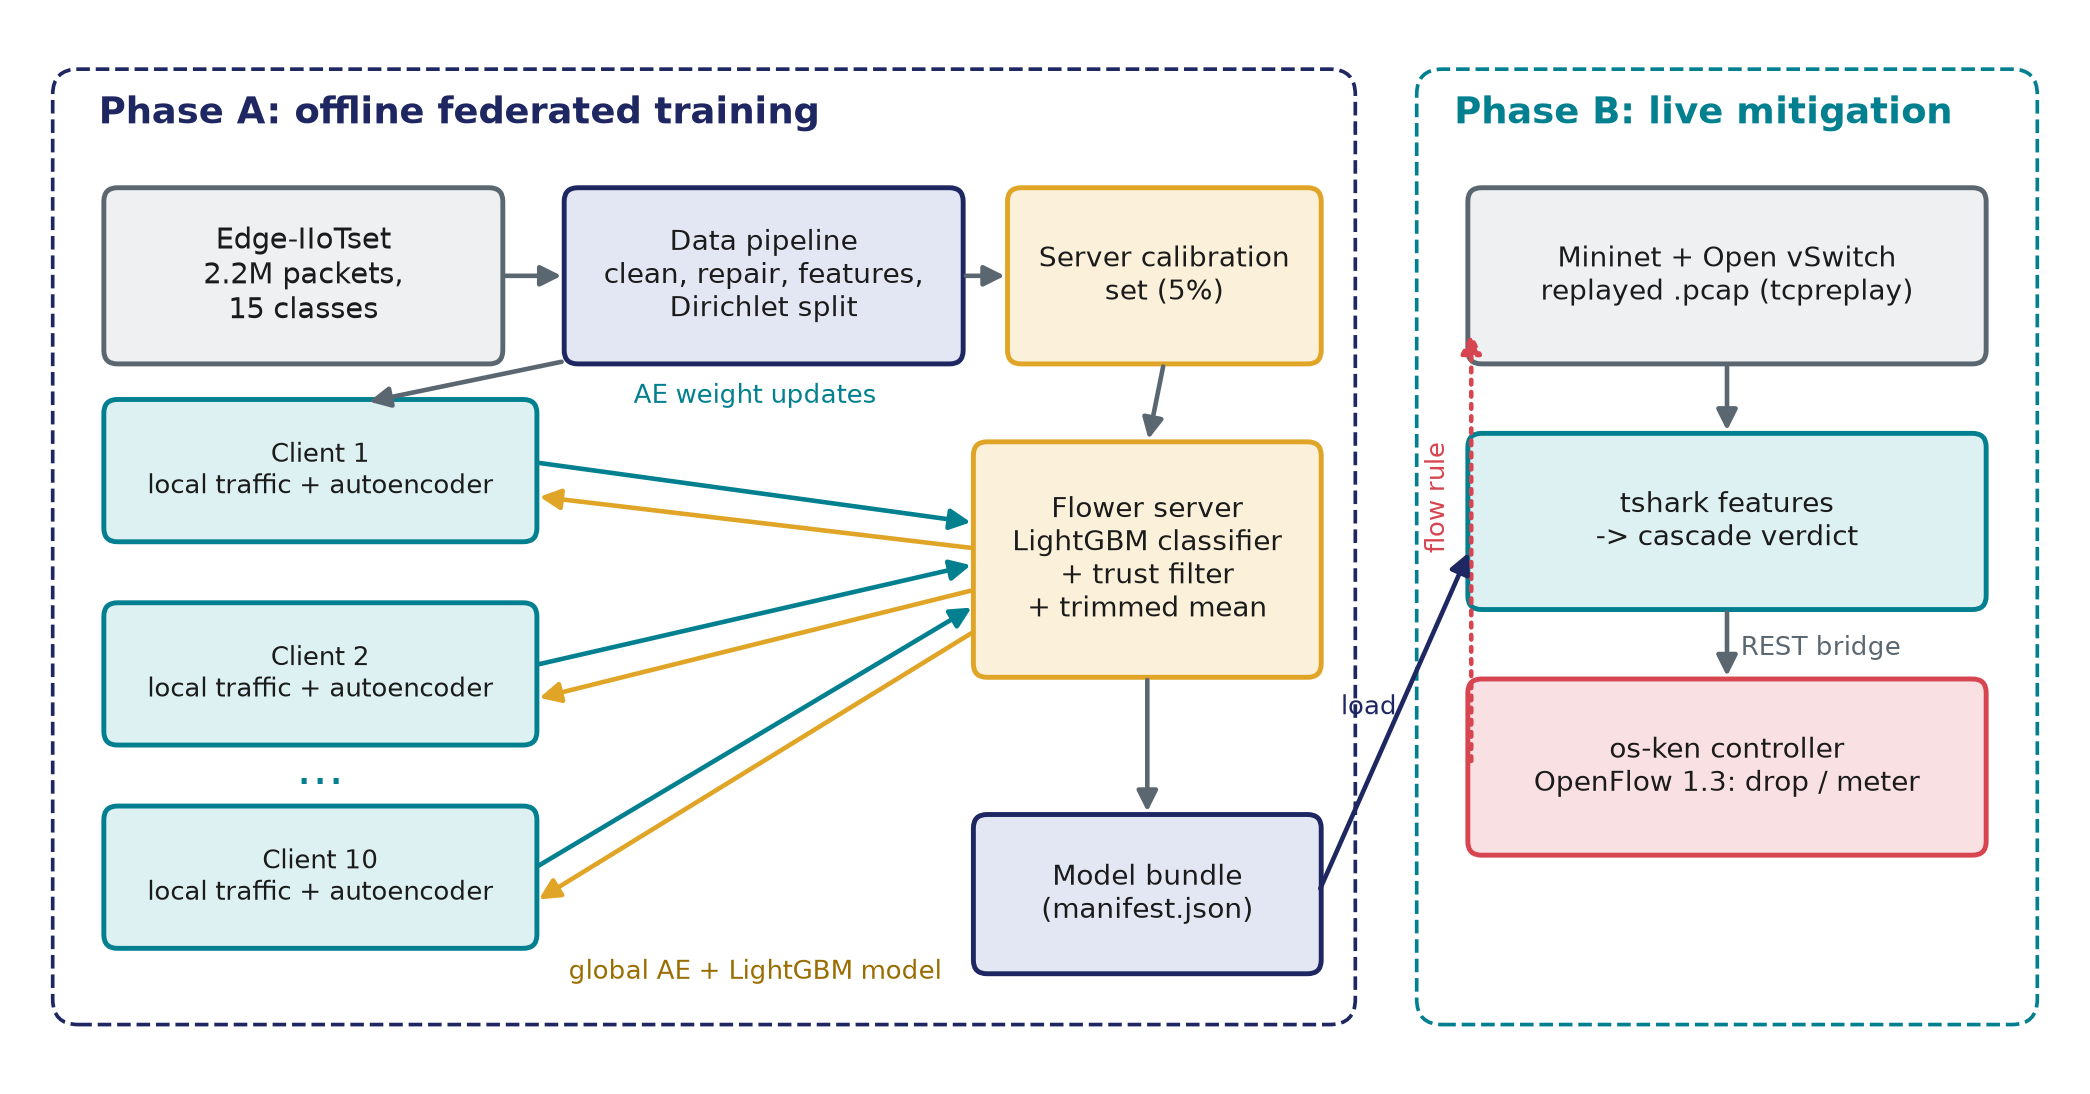
\includegraphics[width=\linewidth]{figures/high_level_design.png}
\caption{High-level design of FL-IDS}
\label{fig:hld}
\end{figure}

\section{Tools and Techniques}
\begin{itemize}
  \item \textbf{LightGBM}~\cite{ke2017lightgbm}: histogram-based gradient-boosted decision trees, used as the first-stage multi-class classifier. Trees work directly on raw feature values, so each client's local normalisation cannot distort the classifier's split thresholds.
  \item \textbf{Autoencoder (PyTorch)}: a dense network $130\rightarrow32\rightarrow16\rightarrow8\rightarrow16\rightarrow32\rightarrow130$ with ReLU activations and a linear output, 9{,}834 parameters in total (7{,}299 with the original 91 features). It learns to reconstruct benign traffic, so a high reconstruction error indicates unusual traffic.
  \item \textbf{Flower}: the federated learning framework. A custom strategy, \texttt{TrustFiltered\-Strategy} (a subclass of FedAvg), implements the trust filter and trimmed-mean aggregation.
  \item \textbf{Cosine similarity, median absolute deviation (MAD) and exponential moving average (EMA)}: the statistics used by the trust filter.
  \item \textbf{Mininet, Open vSwitch, os-ken}: network emulation, the software switch, and the OpenFlow~1.3 controller (os-ken is the maintained fork of Ryu).
  \item \textbf{TShark and tcpreplay}: extracting the dataset's fields from live packets, and replaying captures into the emulated network.
  \item \textbf{Streamlit}: the live dashboard.
\end{itemize}

\section{Data Set With Explanation}
\textbf{Edge-IIoTset}~\cite{ferrag2022edge} was generated on a seven-layer IoT/IIoT testbed (cloud, network functions virtualisation, blockchain, fog, SDN, edge and IoT/IIoT perception layers) with more than ten kinds of sensors, including temperature, humidity, water level, pH, soil moisture, heart rate and flame sensors. They communicate over MQTT and Modbus/TCP. The authors' ML-ready file, \texttt{DNN-EdgeIIoT-dataset.csv}, has 2{,}219{,}201 rows and 63 columns: 61 packet-level fields extracted with tshark, plus \texttt{Attack\_label} and \texttt{Attack\_type}. The 24 per-device and per-attack \texttt{.pcap} captures are also used, for Phase B replay and for repairing corrupted rows.

There are 15 classes: Normal and 14 attacks in five groups. Table~\ref{tab:classes} gives the class sizes after cleaning (current code, before the new features are added).

\begin{table}[H]
\centering
\renewcommand{\arraystretch}{1.15}
\begin{tabular}{|l|l|r|r|}
\hline
\textbf{Group} & \textbf{Class} & \textbf{Rows} & \textbf{\%} \\ \hline
-- & Normal & 1{,}363{,}998 & 71.42 \\ \hline
DoS/DDoS & DDoS\_UDP & 121{,}567 & 6.37 \\
 & DDoS\_ICMP & 67{,}939 & 3.56 \\
 & DDoS\_TCP & 50{,}062 & 2.62 \\
 & DDoS\_HTTP & 48{,}544 & 2.54 \\ \hline
Injection & SQL\_injection & 50{,}826 & 2.66 \\
 & Uploading & 36{,}807 & 1.93 \\
 & XSS & 15{,}066 & 0.79 \\ \hline
Information gathering & Vulnerability\_scanner & 50{,}026 & 2.62 \\
 & Port\_Scanning & 19{,}977 & 1.05 \\
 & Fingerprinting & 853 & 0.04 \\ \hline
Malware & Password & 49{,}933 & 2.61 \\
 & Backdoor & 24{,}026 & 1.26 \\
 & Ransomware & 9{,}689 & 0.51 \\ \hline
Man-in-the-middle & MITM & 406 & 0.02 \\ \hline
\multicolumn{2}{|l|}{\textbf{Total}} & \textbf{1{,}909{,}719} & \\ \hline
\end{tabular}
\caption{Class distribution after cleaning (91 base features)}
\label{tab:classes}
\end{table}

\subsection{Data-quality problems found and fixed}\label{sec:dataquality}
\begin{enumerate}
  \item \textbf{Placeholder label leak.} In the categorical columns, the ``field does not apply'' value is written as \texttt{0} in some source captures and \texttt{0.0} in others, and the spelling follows the label. In \texttt{mqtt.topic}, \texttt{mqtt.conack.flags}, \texttt{mqtt.protoname} and \texttt{dns.qry.name.len}, every Normal row uses \texttt{0} and every attack row \texttt{0.0}. After one-hot encoding, the single column \texttt{mqtt.topic\_0.0} separates benign from attack with an AUROC of 1.0. Both spellings are mapped to \texttt{0} before encoding, after which the strongest single feature has an AUROC of about 0.71. A test guards that no single feature exceeds 0.9.
  \item \textbf{Column-shifted MITM rows.} In the authors' MITM rows, values sit under the wrong column names (for example, their \texttt{tcp.seq} is really \texttt{udp.time\_delta}, with 1.000 agreement). These rows are replaced by re-extracting the authors' own MITM capture with the same field list (1{,}214 rows replaced by 1{,}229).
  \item \textbf{TShark version drift.} Newer tshark prints booleans as \texttt{True}/\texttt{False} and shortens hexadecimal values. Without a fix, this silently zeroed \texttt{tcp.flags.ack} on every live packet in Phase B. Live extraction maps both back to the authors' format.
\end{enumerate}

\subsection{Preprocessing}
Sixteen columns are dropped, following the dataset authors' recipe: identifiers, timestamps, raw payloads and ports, plus \texttt{Attack\_label}, which is fully determined by \texttt{Attack\_type}. Seven nominal columns are one-hot encoded, giving \textbf{91 base features}. Exact duplicate rows are removed (309{,}497 rows), leaving 1{,}909{,}719 rows.

\subsection{New features for the classifier}
Profiling the dropped columns explained why the application-layer attacks were hard to classify. In the SQL\_injection, XSS, Uploading and Password classes, only 5--17\% of packets carry any HTTP content. The rest are content-free TCP handshake and acknowledgement packets to port~80 on the same web server, which look the same whichever attack produced them. Three groups of features were therefore added. IP addresses, absolute time and ephemeral client ports are \emph{never} used as features, because each of them identifies the capture file and hence the label.
\begin{enumerate}
  \item \textbf{Service port (1 feature):} the server side of a connection, $\min(\text{ports} < 32768)$, or $-1$ if there is none (for example ICMP or ARP).
  \item \textbf{Content features (18):} decoded payload length, byte entropy, printable fraction, HTTP request flag, HTTP status code, header count, \texttt{X-} header count, URI length, parameter count, percent-encoding count, file-data length, special-character count, and counts of six generic attack-signature keyword groups (SQL, script/XSS, upload, authentication, traversal/command, scanner tool names).
  \item \textbf{Flow features (20):} packets are grouped into flows by (IP pair, protocol, port pair) in capture order. A new flow starts after a 60\,s idle gap or once a flow has been active for 120\,s, CICFlowMeter's default active timeout~\cite{sharafaldin2018cicids}. Every packet in a flow receives the flow's packet count, duration, packet rate, payload sum/maximum/non-zero share, HTTP request count, maximum status code, SYN, FIN and RST counts, maximum entropy, maximum URI length and keyword totals. IP addresses and times are used only to group packets, never as features.
\end{enumerate}
With all three groups there are 130 features and 1{,}985{,}768 unique rows.

\section{Flow Chart Of Methodology From Start To End}
Figure~\ref{fig:flow} shows the complete sequence of steps, from loading the dataset to verifying the mitigation rule.
\begin{figure}[H]
\centering
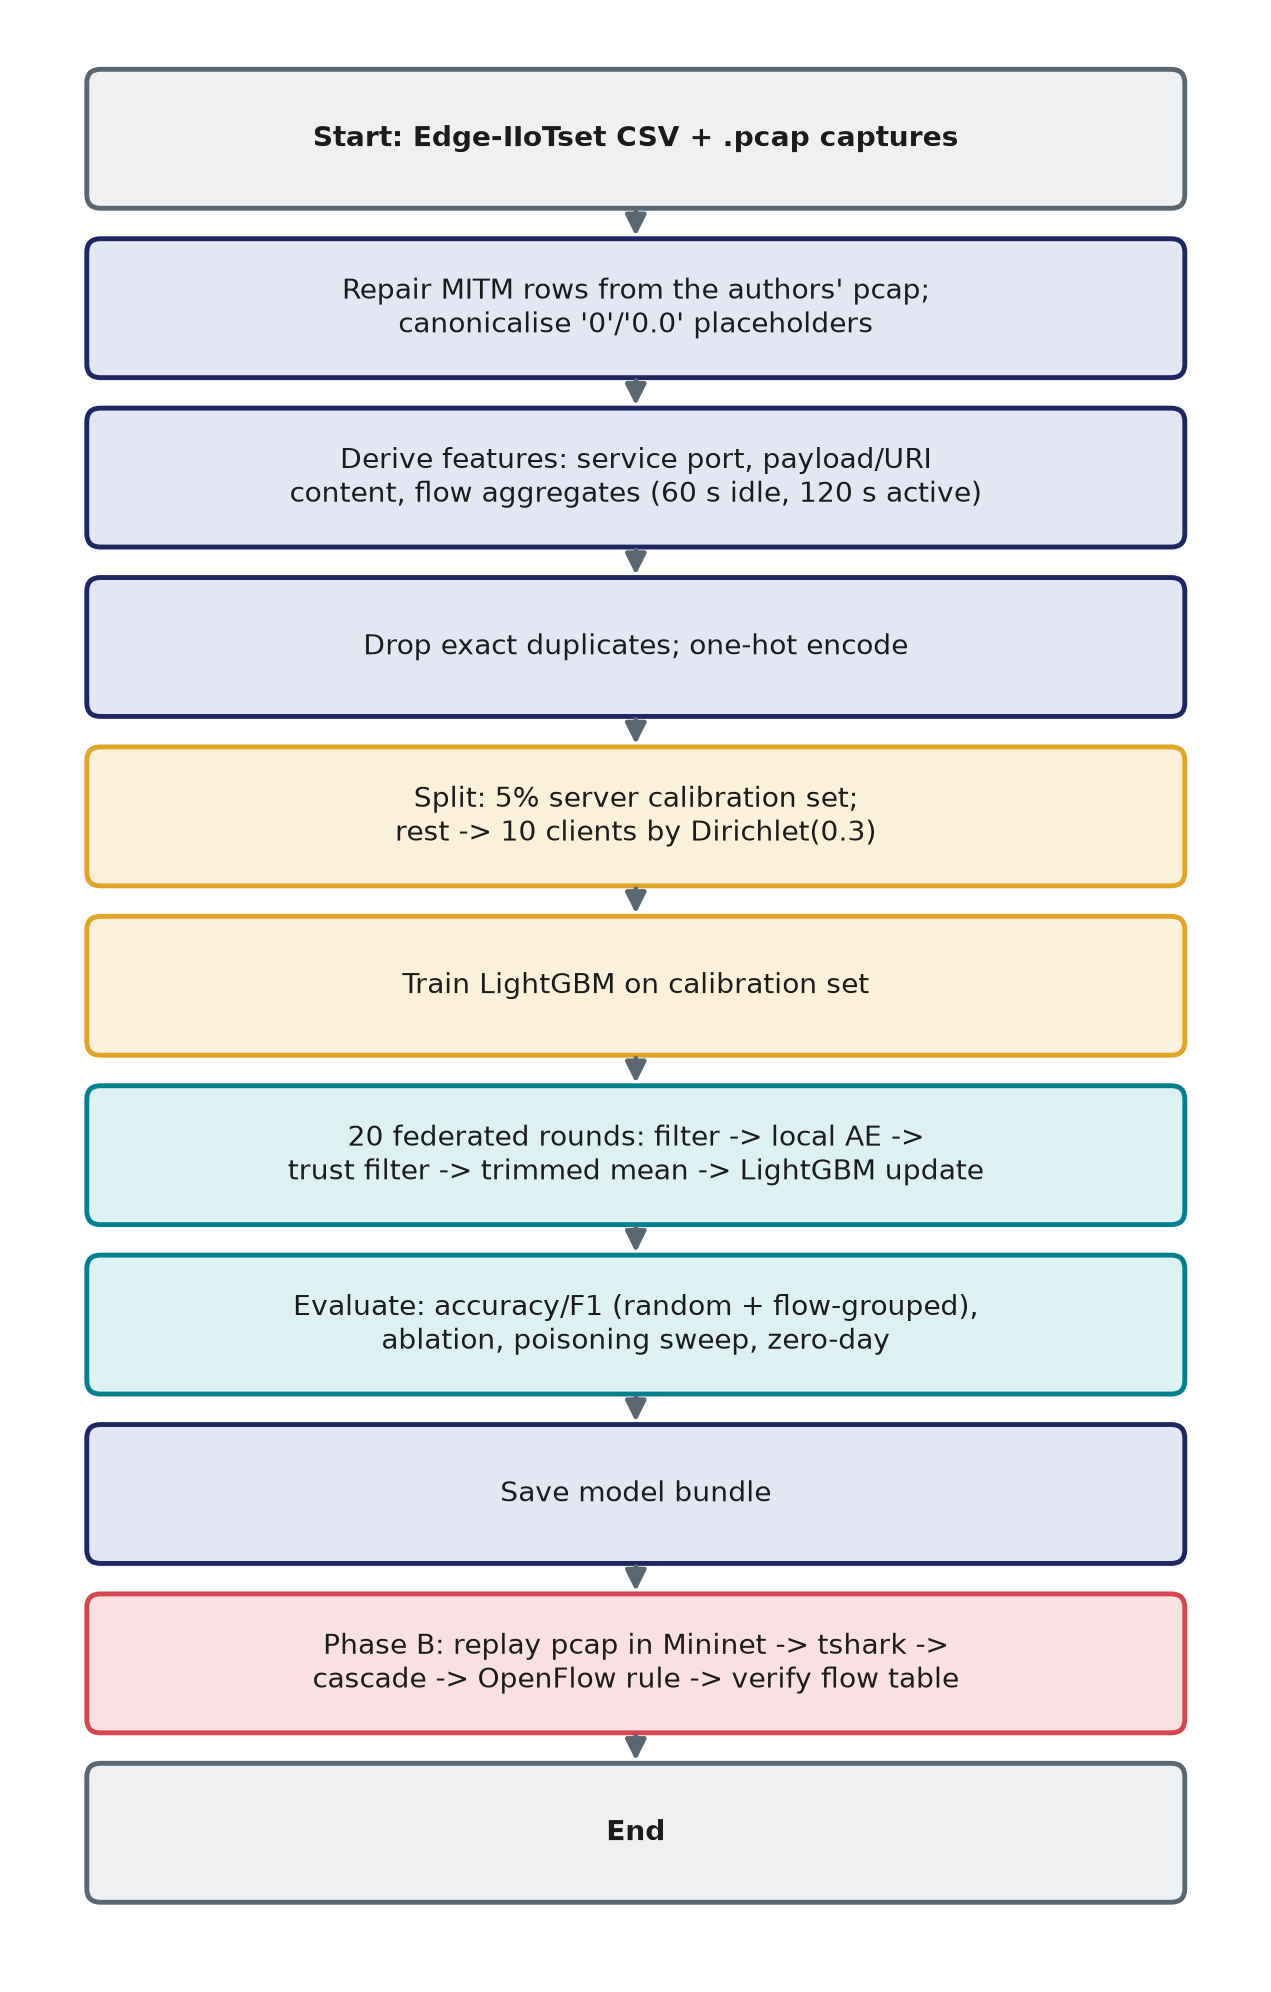
\includegraphics[width=0.62\linewidth]{figures/methodology_flowchart.png}
\caption{Flow chart of the methodology}
\label{fig:flow}
\end{figure}

\section{Explanation Of Methodology In Details With Equations And Formulae}

\subsection{How much data each part uses}
Every packet of the dataset is cleaned and given the new features (2{,}219{,}216 rows, 1{,}985{,}768 unique after de-duplication). How many of them each model trains on differs, and Table~\ref{tab:datascale} lists it. The classifier that meets the accuracy target is trained on most of the data. The federated system uses a smaller share, because its pool is capped at 60{,}000 rows to keep the roughly 150 evaluation runs practical.
\begin{table}[H]
\centering
\small
\renewcommand{\arraystretch}{1.2}
\begin{tabular}{|>{\raggedright\arraybackslash}p{4.4cm}|>{\raggedright\arraybackslash}p{4.7cm}|>{\raggedright\arraybackslash}p{4.7cm}|}
\hline
\textbf{Part} & \textbf{Trained on} & \textbf{Evaluated on} \\ \hline
Final classifier (accuracy target) & 1{,}429{,}825 rows (72\%), plus 158{,}870 for early stopping (8\%) & 397{,}073 unseen rows (20\%); whole connections held out \\ \hline
Same classifier, 5\% share only & 89{,}359 rows, plus 9{,}929 for early stopping & the same 397{,}073 rows \\ \hline
Federated: server bootstrap classifier & 79{,}430 rows (calibration set) & 19{,}858 rows held back \\ \hline
Federated: client autoencoders & 45{,}474 rows across 10 clients (736 to 11{,}549 each), plus 5{,}530 benign rows for thresholds & 8{,}996 client test rows \\ \hline
\end{tabular}
\caption{Training and evaluation rows for each part (130 features, seed 42)}
\label{tab:datascale}
\end{table}
The 5\%-only row shows that the federated bootstrap loses little from its smaller training set: 99.7\% accuracy and 0.979 macro F1 on the same 397{,}073 test rows, against 0.983 for the full classifier.

\subsection{Non-IID partition and per-client normalisation}
A stratified 5\% of the rows is held on the server as the calibration set. The remaining federated pool (subsampled to 60{,}000 rows to keep the roughly 150 evaluation runs practical) is split across $N=10$ clients. For each class $k$ a proportion vector is drawn,
\begin{equation}
  \mathbf{p}_k \sim \mathrm{Dir}(\alpha\mathbf{1}_N), \qquad \alpha = 0.3,
\end{equation}
and the class's rows are divided in those proportions~\cite{hsu2019noniid}. Smaller $\alpha$ gives more skew. Each client keeps 15\% as a test slice and 15\% of its benign remainder as a benign validation slice. For the autoencoder only, client $i$ standardises features with its own training mean $\mu_i$ and standard deviation $\sigma_i$, clipped at $\pm10$:
\begin{equation}
  \tilde{x} = \mathrm{clip}\!\left(\frac{x-\mu_i}{\sigma_i},\,-10,\,10\right).
\end{equation}
The clip is needed because a counter feature can barely vary inside one skewed shard. Without it, one client's benign validation loss stayed near 400 for 20 rounds; with it, the loss fell to 0.0146.

\subsection{Stage 1: LightGBM classifier}
LightGBM builds an additive model of $T$ trees per class, $F_k(\mathbf{x}) = \sum_{t=1}^{T} f_{t,k}(\mathbf{x})$, with class probabilities
\begin{equation}
  P(y=k\mid\mathbf{x}) = \frac{e^{F_k(\mathbf{x})}}{\sum_{j=1}^{15} e^{F_j(\mathbf{x})}},
\end{equation}
trained by minimising the weighted multi-class log loss
\begin{equation}
  \mathcal{L} = -\frac{1}{\sum_n w_n}\sum_{n} w_{n}\,\log P(y=y_n\mid\mathbf{x}_n) + \lambda_2 \sum_{t}\lVert \mathbf{v}_t\rVert^2 ,
\end{equation}
where $\mathbf{v}_t$ are leaf values and $\lambda_2 = 1$. The sample weight $w_n$ is a square-root inverse class frequency, recomputed for every training set (the bootstrap and each incremental update),
\begin{equation}
  w_n = \sqrt{\frac{\max_j N_j}{N_{y_n}}},
\end{equation}
so a rare class such as Fingerprinting counts more without being blown up the way full inverse-frequency weights would. In the federated pipeline the classifier uses 300 rounds, learning rate 0.05 and 31 leaves, trained deterministically on one thread so runs are reproducible. The stand-alone accuracy experiments of Section~5.1 used 63 leaves, learning rate 0.1, feature and bagging fractions of 0.8, and early stopping after 50 rounds without improvement on a 10\% validation split.

\subsection{Stage 2: autoencoder and threshold}
Each client trains the autoencoder $g_\theta$ on the rows the current classifier passes (predicted Normal, or an attack with probability below 0.7). It minimises the mean squared reconstruction error
\begin{equation}
  e(\mathbf{x}) = \frac{1}{d}\sum_{j=1}^{d}\big(\tilde{x}_j - g_\theta(\tilde{\mathbf{x}})_j\big)^2
\end{equation}
with Adam (learning rate $10^{-3}$, 5 local epochs, batch size 64). The client's threshold is recomputed every round as the 97th percentile of $e$ on its benign validation slice, $\tau_i = Q_{0.97}\{e(\mathbf{x}) : \mathbf{x}\in V_i\}$.

\subsection{Cascade decision rule}
Figure~\ref{fig:cascade} shows the shared decision rule. With $\hat{k}=\arg\max_k P(k\mid\mathbf{x})$ and $p = P(\hat{k}\mid\mathbf{x})$:
\begin{equation}
\text{label}(\mathbf{x}) =
\begin{cases}
  \hat{k} & \text{if } \hat{k}\neq\text{Normal and } p \geq 0.7,\\
  \text{anomalous} & \text{else if } e(\mathbf{x}) > \tau_i,\\
  \text{benign} & \text{otherwise,}
\end{cases}
\end{equation}
with confidence $p$ for a known attack and $\mathrm{clip}(e/\tau_i - 1,\,0,\,1)$ for an anomaly.
\begin{figure}[H]
\centering
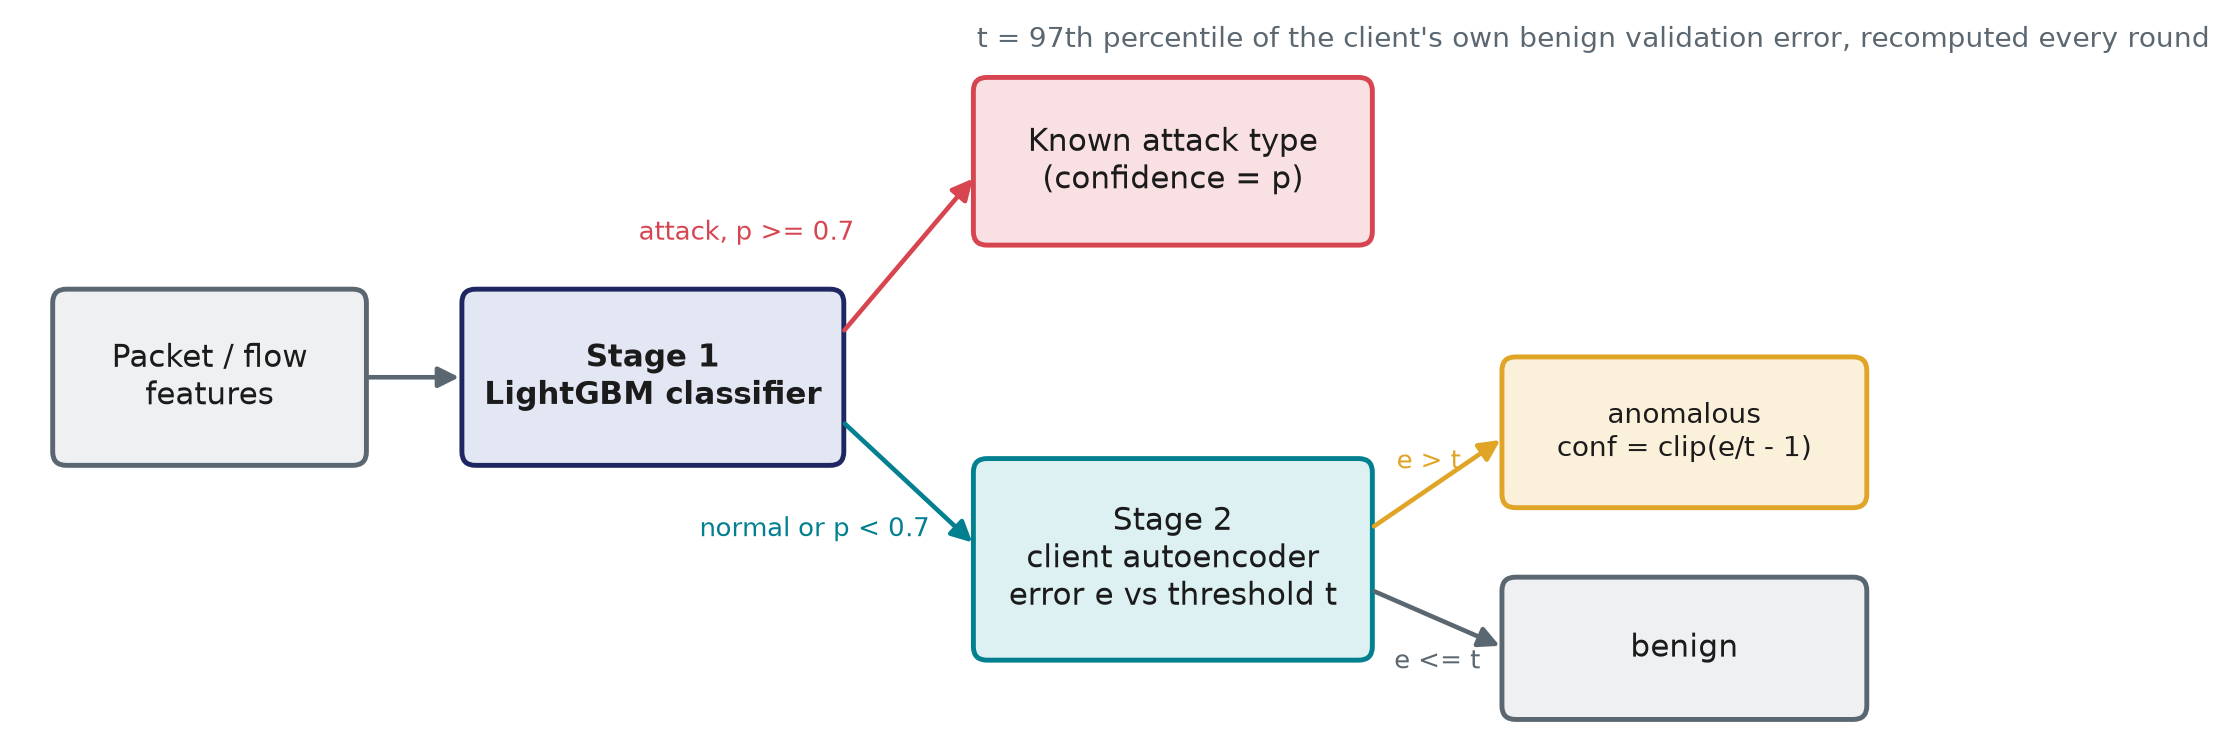
\includegraphics[width=0.92\linewidth]{figures/cascade_rule.png}
\caption{Two-stage cascade decision rule}
\label{fig:cascade}
\end{figure}

\subsection{Trust filter and robust aggregation}
Let $\mathbf{w}^{(r)}$ be the global weights at the start of round $r$ and $\mathbf{w}_i$ client $i$'s weights after local training. The filter works on \emph{deltas} $\Delta_i = \mathbf{w}_i - \mathbf{w}^{(r)}$. The reference direction is the coordinate-wise median $\mathbf{m} = \mathrm{median}_i(\Delta_i)$, and each client's similarity is
\begin{equation}
  s_i = \frac{\Delta_i\cdot\mathbf{m}}{\lVert\Delta_i\rVert\,\lVert\mathbf{m}\rVert}.
\end{equation}
Trust is a running average, starting at $T_i=1$:
\begin{equation}
  T_i \leftarrow (1-\beta)\,T_i + \beta\,\frac{s_i+1}{2}, \qquad \beta = 0.3 .
\end{equation}
Client $i$ is excluded in round $r$ if any of these holds:
\begin{equation}
  s_i < \tilde{s} - 3\,\mathrm{MAD}(s) \quad\text{or}\quad s_i < 0 \quad\text{or}\quad T_i < 0.5 ,
\end{equation}
where $\tilde{s}$ is the median similarity. Surviving deltas are clipped to twice the median norm $\nu$,
\begin{equation}
  \Delta_i' = \Delta_i\cdot\min\!\left(1,\ \frac{2\nu}{\lVert\Delta_i\rVert}\right),
\end{equation}
and combined coordinate-wise with a 15\% trimmed mean, which drops the largest and smallest $\lfloor0.15\,n\rfloor$ values in each coordinate:
\begin{equation}
  \mathbf{w}^{(r+1)} = \mathbf{w}^{(r)} + \mathrm{TrimMean}_{0.15}\big(\{\Delta_i'\}\big).
\end{equation}
The test attacker trains honestly and then sends $-5\Delta_i$ (sign flip, amplified five times), while claiming the largest client's example count. Figure~\ref{fig:round} summarises one round.
\begin{figure}[H]
\centering
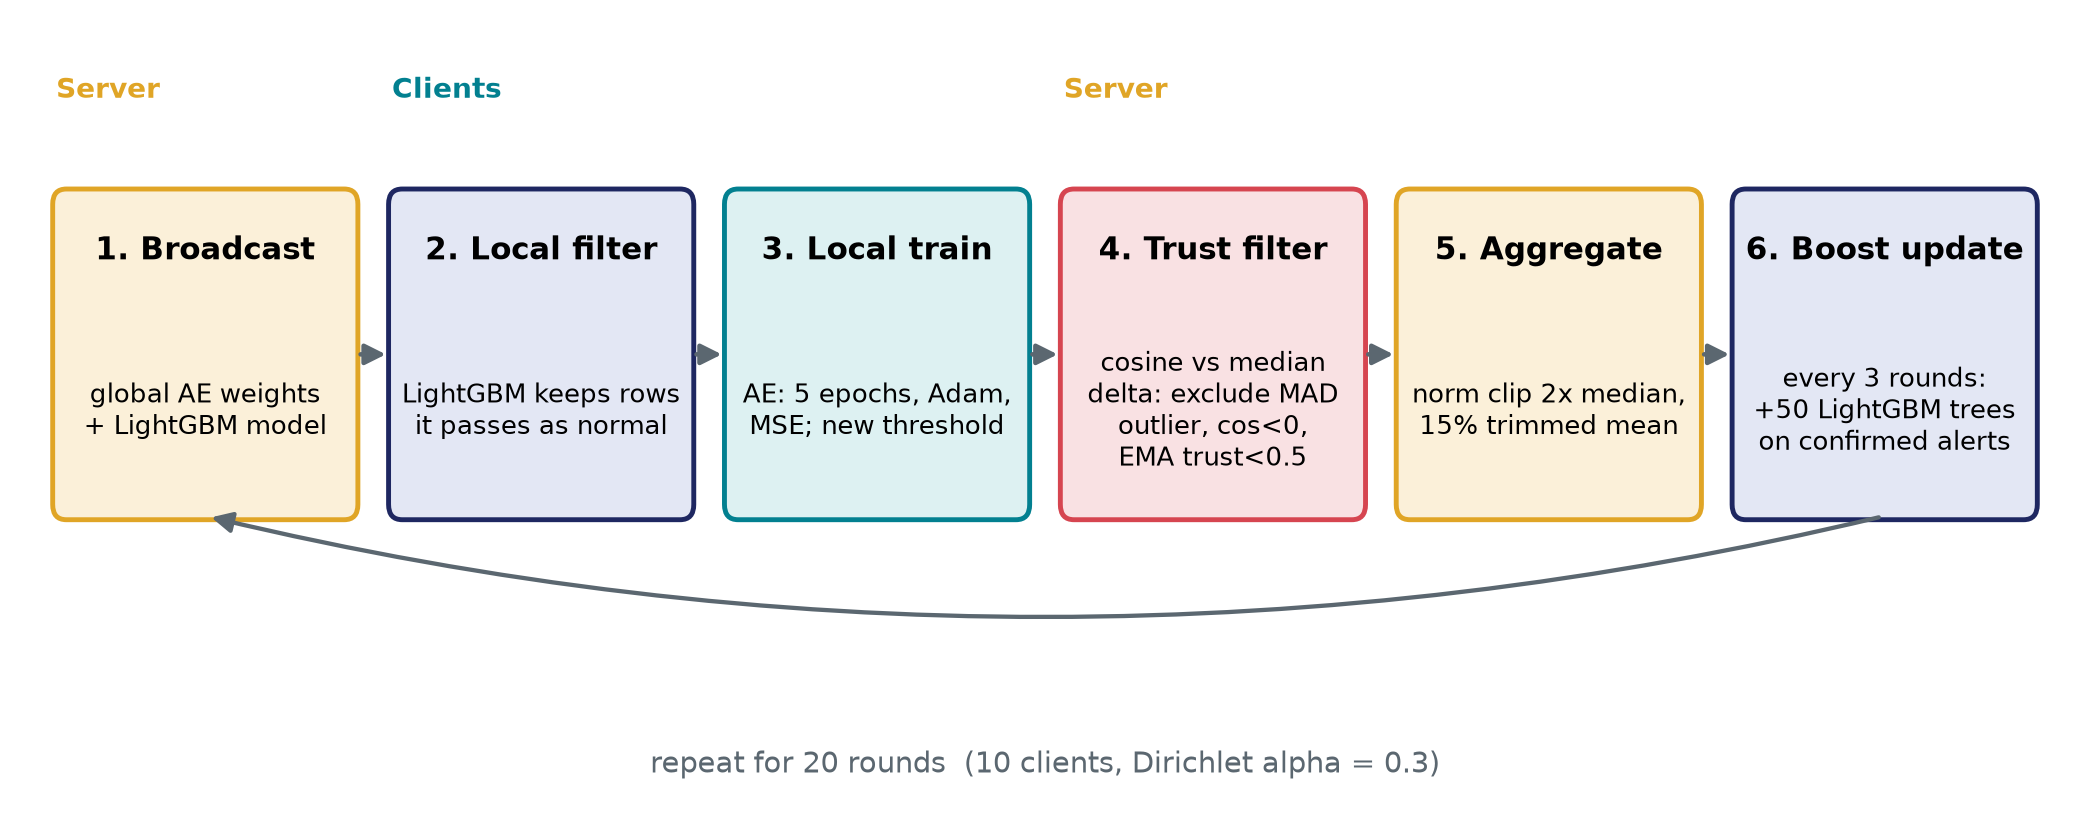
\includegraphics[width=\linewidth]{figures/fl_round.png}
\caption{One federated round}
\label{fig:round}
\end{figure}

\subsection{Incremental classifier update}
Every 3 rounds, each client that survived the filter surfaces up to 50 rows its autoencoder flagged, with analyst-confirmed labels. The server continues training LightGBM with 50 more trees on the calibration set plus all collected alerts, or retrains from scratch if the alerts contain a class the model has never seen. This relaxes the ``no raw traffic leaves a client'' rule for these capped, confirmed alerts only, and is reported as a privacy trade-off.

\subsection{SDN mitigation}
In Phase B, Mininet creates one host per federated client on one Open vSwitch switch, controlled by os-ken over OpenFlow~1.3. A real attack capture is replayed with tcpreplay. TShark extracts all 61 of the dataset's fields, the service-port, content and flow features are derived from the capture with the same code as in training, each row is scored with that host's own scaler and threshold, and the most frequent non-benign label becomes the device verdict. A Flask bridge maps the verdict to an action: \emph{block} (a drop rule on the source IP) if confidence $\geq0.85$, \emph{rate-limit} (an OpenFlow meter) if $\geq0.5$, otherwise allow. The installed rule is then read back from the switch's flow table to confirm it.

\subsection{Evaluation metrics}
With $TP_k$, $FP_k$, $FN_k$ counted per class $k$ over $K$ classes:
\begin{align}
  \text{Accuracy} &= \frac{\#\text{correct}}{\#\text{test rows}}, &
  P_k &= \frac{TP_k}{TP_k+FP_k}, &
  R_k &= \frac{TP_k}{TP_k+FN_k},\\
  F1_k &= \frac{2P_kR_k}{P_k+R_k}, &
  \text{Macro F1} &= \frac{1}{K}\sum_{k}F1_k .
\end{align}
Because 71\% of traffic is benign, accuracy alone hides poor results on rare attacks, so macro F1 is reported next to it. A class with no rows in a test split (MITM is a single flow) is left out of that split's macro average. Two splits are used: a \textbf{stratified random 80/20 split} of rows, and a stricter \textbf{flow-grouped 80/20 split} (stratified group k-fold), in which every flow lies entirely in training or entirely in test, so the model cannot score well by memorising connections. The \textbf{ambiguity ceiling}, the accuracy of an oracle that gives every distinct feature vector its majority label, shows how separable the classes are with a given feature set. For the federated system, attack macro-recall, benign false-positive rate, zero-day macro-recall (leave one attack class out of all training data, then score it) and malicious-client survival rate are also reported.

\chapter{Results and Discussion}\label{chap:results}
All numbers below come from logged runs on the hardware in Chapter~3. Unless stated otherwise, the seed is 42.

\section{Classifier accuracy}
The project requirement was at least 95\% accuracy and at least 0.95 macro F1. The earlier classifier comparison, on a 500{,}000-row class-balanced sample of the base features, gave 0.891 accuracy and 0.887 macro F1. On all 1.9 million rows with the natural class distribution, the same base features give 0.964 accuracy but still only 0.887 macro F1, because the application-layer attacks are confused with each other.

The final classifier is trained on 1{,}429{,}825 packets and tested on 397{,}073 packets from connections it never saw (Table~\ref{tab:datascale}).

\subsection{Ambiguity ceiling}
Before tuning the model, we measured how many rows are impossible to separate with each feature set (Table~\ref{tab:ceiling}). With the 91 base features, 2.31\% of rows share an identical feature vector with a row of a different class, which caps macro recall at 0.969 for \emph{any} per-packet classifier. The new features bring the ambiguous share down to 0.01\%.
\begin{table}[H]
\centering
\renewcommand{\arraystretch}{1.2}
\begin{tabular}{|l|c|c|c|c|}
\hline
\textbf{Feature set} & \textbf{Features} & \textbf{Ambiguous} & \textbf{Ceiling acc.} & \textbf{Ceiling macro rec.} \\ \hline
Base & 91 & 2.31\% & 0.9875 & 0.9692 \\ \hline
+ service port & 92 & 0.29\% & 0.9985 & 0.9940 \\ \hline
+ content + flow & 130 & 0.01\% & 0.9999 & 0.9997 \\ \hline
\end{tabular}
\caption{Ambiguity ceiling per feature set (all rows, after de-duplication)}
\label{tab:ceiling}
\end{table}

\subsection{Effect of each feature group}
Table~\ref{tab:progression} and Figure~\ref{fig:progression} add the feature groups one at a time, on the strict flow-grouped split. The service port mainly fixes Normal versus attack traffic. The content features add little on their own, because only a small share of packets carries content. The flow features give the largest jump, because they pass a connection's content and behaviour on to its content-free packets. Class weighting then stabilises the rare Fingerprinting class.
\begin{table}[H]
\centering
\renewcommand{\arraystretch}{1.2}
\begin{tabular}{|l|c|c|c|c|}
\hline
 & \multicolumn{2}{c|}{\textbf{Random split}} & \multicolumn{2}{c|}{\textbf{Flow-grouped split}} \\ \hline
\textbf{Features} & \textbf{Accuracy} & \textbf{Macro F1} & \textbf{Accuracy} & \textbf{Macro F1} \\ \hline
Base (91) & 0.9638 & 0.8868 & 0.9637 & 0.8892 \\ \hline
+ service port (92) & 0.9802 & 0.9245 & 0.9803 & 0.9236 \\ \hline
+ content (110) & 0.9802 & 0.9268 & 0.9802 & 0.9232 \\ \hline
+ flow (130) & 0.9977 & 0.9879 & 0.9975 & 0.9808 \\ \hline
\textbf{+ class weights (final)} & \textbf{0.9976} & \textbf{0.9867} & \textbf{0.9972} & \textbf{0.9828} \\ \hline
\end{tabular}
\caption{Accuracy and macro F1 as feature groups are added (LightGBM, all rows, 80/20)}
\label{tab:progression}
\end{table}
\begin{figure}[H]
\centering
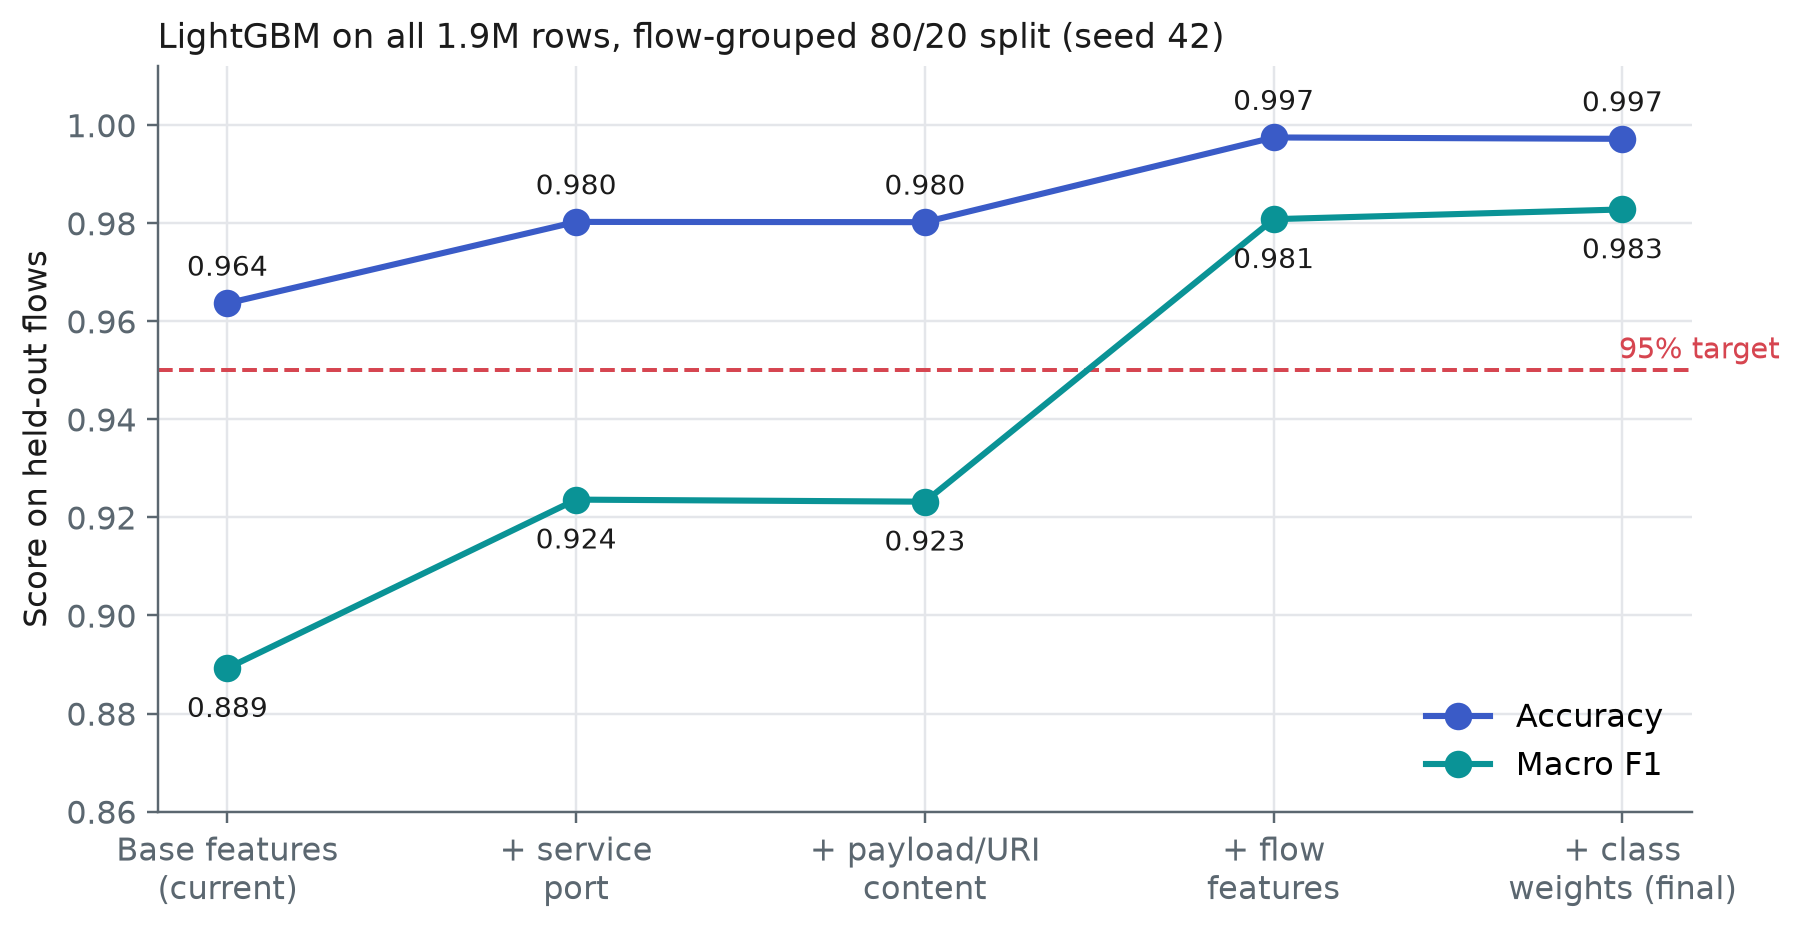
\includegraphics[width=0.92\linewidth]{figures/accuracy_progression.png}
\caption{Accuracy and macro F1 on held-out flows as each feature group is added}
\label{fig:progression}
\end{figure}

\subsection{Robustness across seeds, splits and training size}
Table~\ref{tab:seeds} repeats the final configuration with three seeds on both splits. Accuracy stays between 0.9970 and 0.9977, and macro F1 between 0.9828 and 0.9868. Without class weights, the flow-grouped macro F1 was less stable (0.9808, 0.9560, 0.9521), because the Fingerprinting score depended on which of its 156 flows landed in test. Weighting removes that sensitivity.

\begin{table}[H]
\centering
\renewcommand{\arraystretch}{1.2}
\begin{tabular}{|l|c|c|c|}
\hline
\textbf{Split / seed} & \textbf{42} & \textbf{43} & \textbf{44} \\ \hline
Random: accuracy & 0.9976 & 0.9977 & 0.9976 \\ \hline
Random: macro F1 & 0.9867 & 0.9868 & 0.9866 \\ \hline
Flow-grouped: accuracy & 0.9972 & 0.9971 & 0.9970 \\ \hline
Flow-grouped: macro F1 & 0.9828 & 0.9835 & 0.9851 \\ \hline
\end{tabular}
\caption{Final classifier across seeds}
\label{tab:seeds}
\end{table}

Two further checks were run. \textbf{(a) Same sampling as before:} on a 500{,}000-row capped sample drawn the same way as in the earlier boosting-versus-DL comparison, and with the same training settings for both feature sets, accuracy rises from 0.8902 to 0.9919 and macro F1 from 0.8827 to 0.9900. \textbf{(b) Calibration-set size:} in FL-IDS the server trains LightGBM on only a 5\% calibration set. Trained on 5\% of the rows and tested on held-out flows, the new features give 0.9968 accuracy and 0.9791 macro F1, against 0.9624 and 0.8807 for the base features. The gain therefore carries over to the classifier as the federated system actually trains it.

\subsection{Per-class results}
Figure~\ref{fig:perclass} compares per-class F1 before and after. The biggest gains are on exactly the classes that were weak: Uploading (0.76 to 1.00), DDoS\_HTTP (0.76 to 0.97), SQL\_injection (0.80 to 1.00), Password (0.84 to 0.97), XSS (0.85 to 0.98) and Fingerprinting (0.68 to 0.93). Figure~\ref{fig:cm} shows the remaining confusion: Password and DDoS\_HTTP traffic (both HTTP requests to the same server) and Ransomware versus Backdoor (both on port 4321). MITM is a single ARP flow, so it cannot be scored on the flow-grouped split; on the random split its F1 is 0.994.
\begin{figure}[H]
\centering
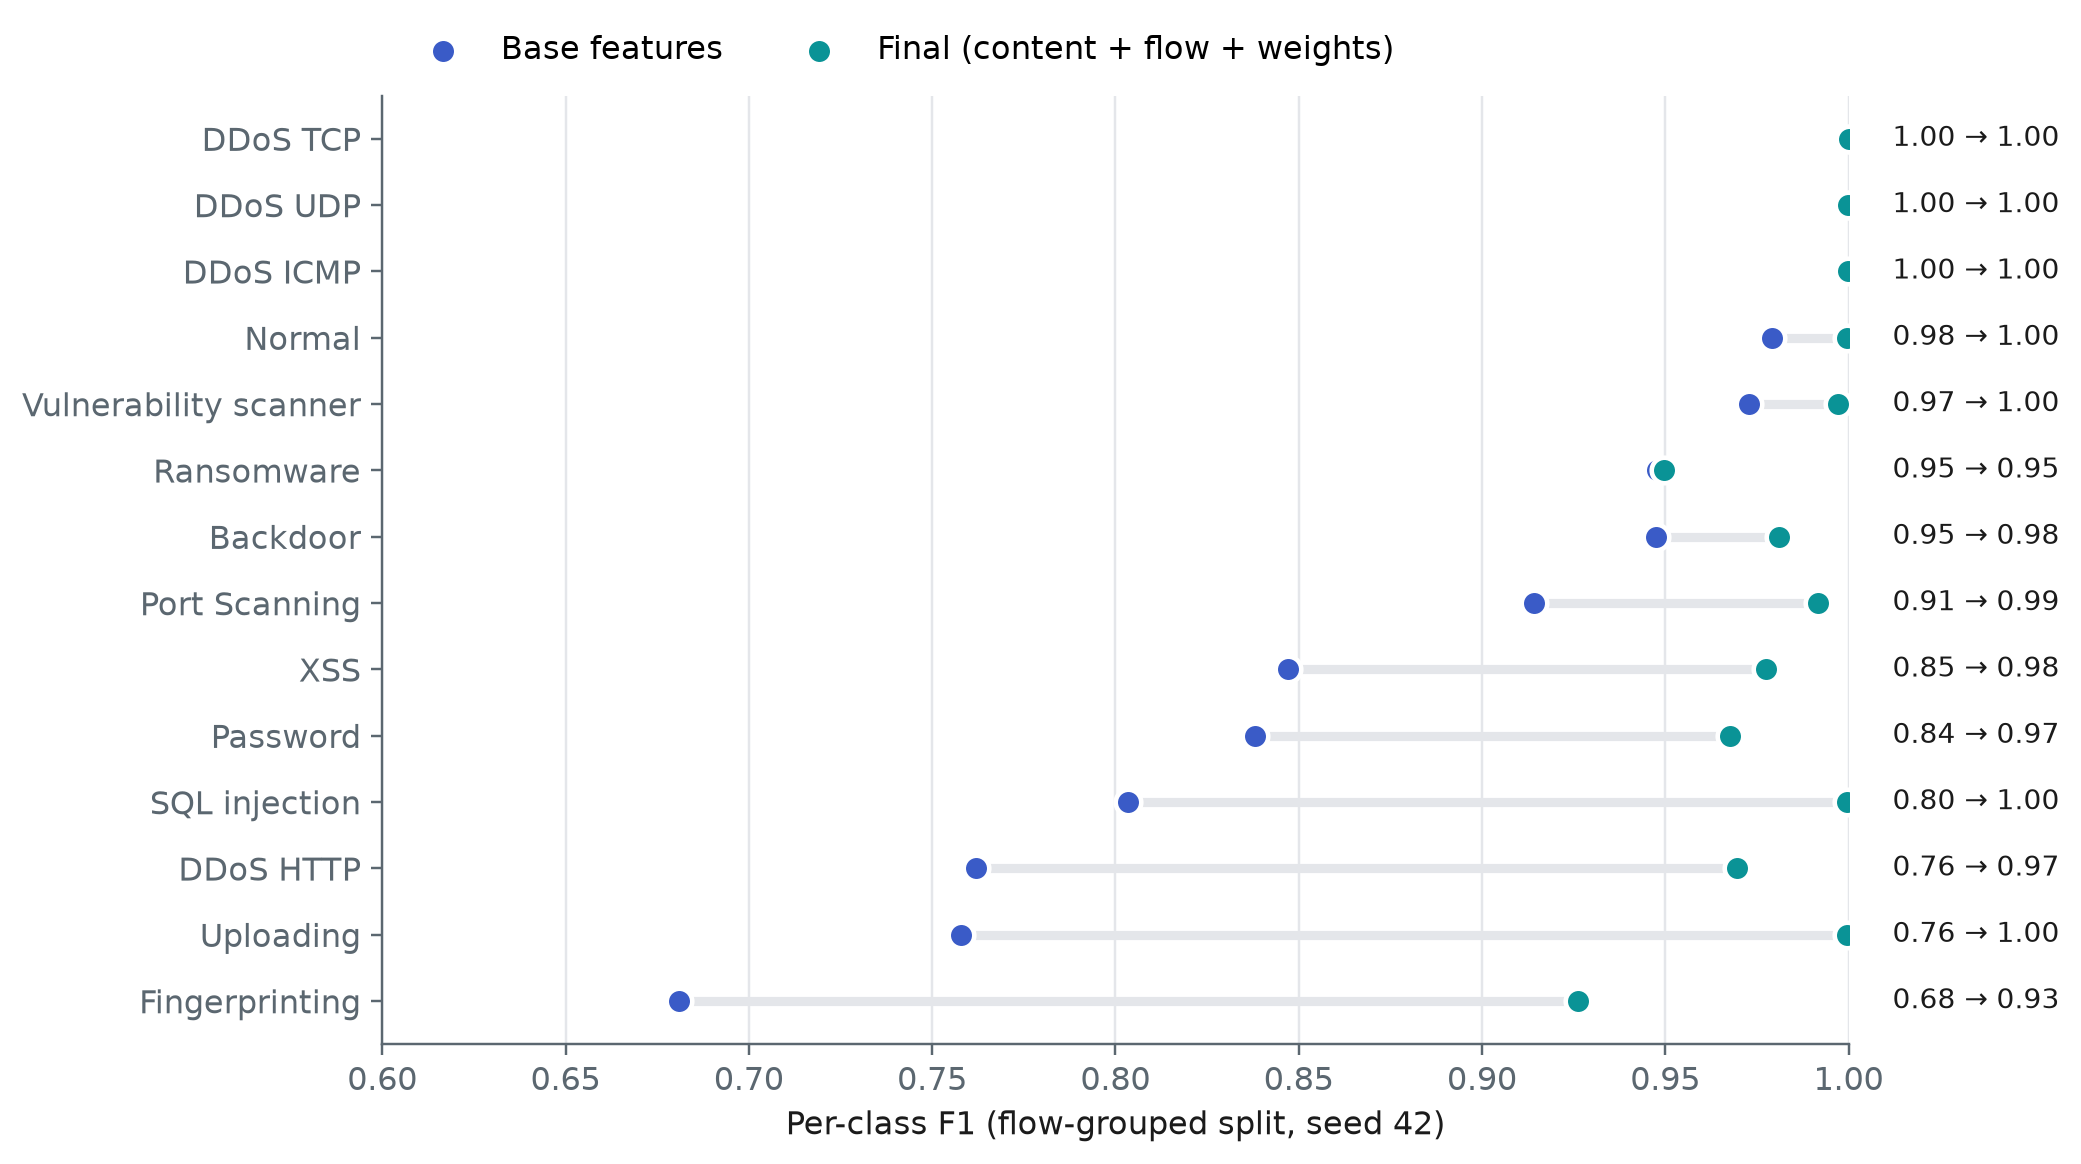
\includegraphics[width=0.88\linewidth]{figures/per_class_f1.png}
\caption{Per-class F1, base features vs.\ final classifier (flow-grouped split)}
\label{fig:perclass}
\end{figure}
\begin{figure}[H]
\centering
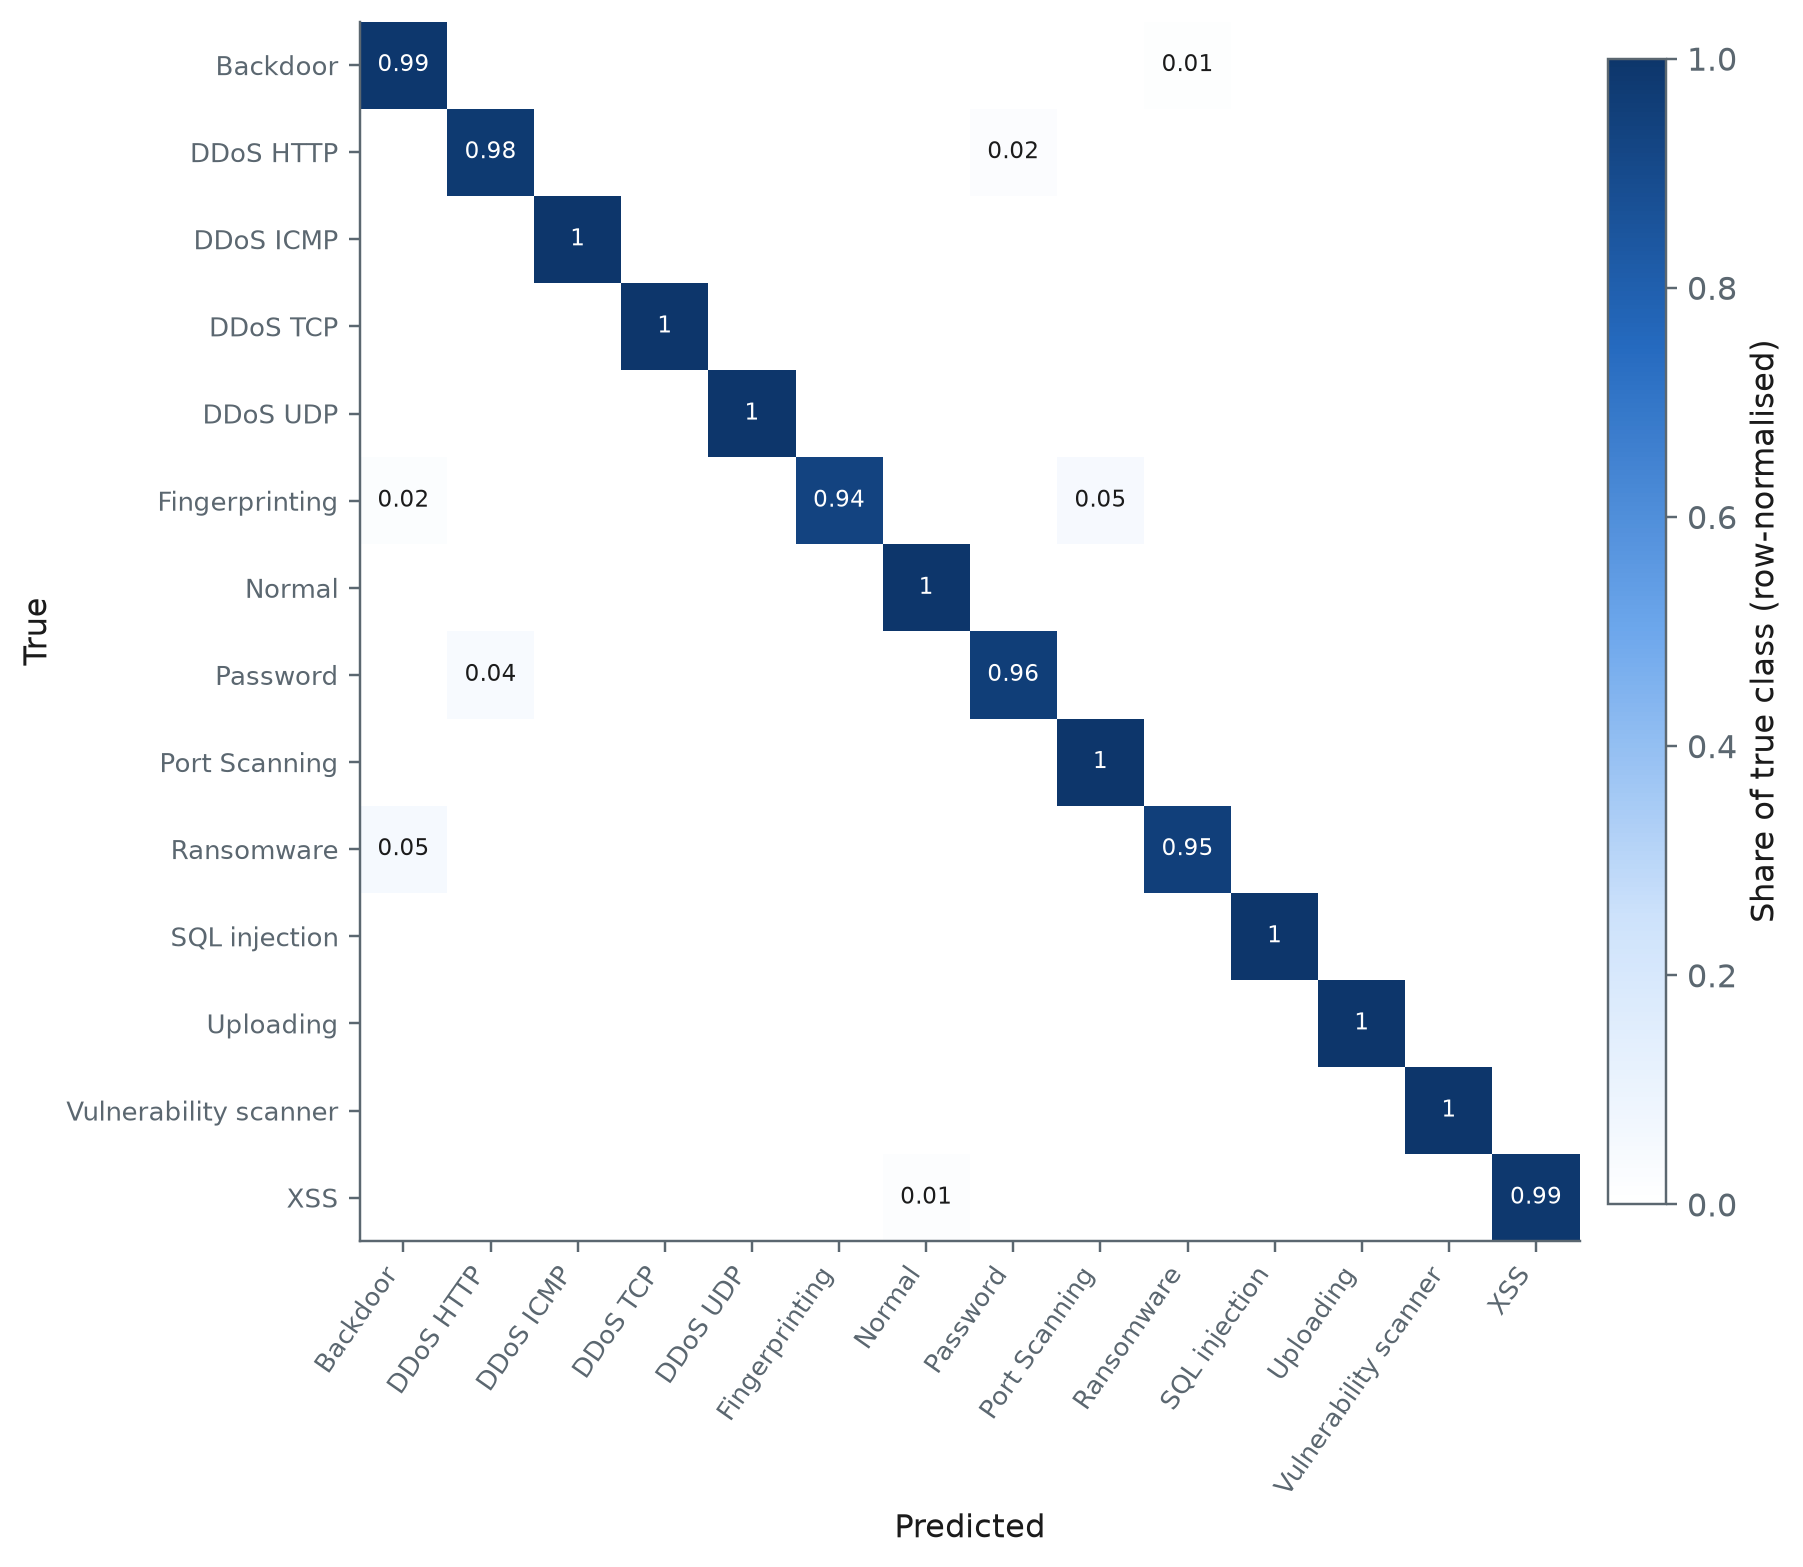
\includegraphics[width=0.8\linewidth]{figures/confusion_final.png}
\caption{Row-normalised confusion matrix of the final classifier (flow-grouped split)}
\label{fig:cm}
\end{figure}

\subsection{Discussion and caveats}
\begin{itemize}
  \item \textbf{Why a flow-grouped split matters.} A random split of packets puts packets of the same connection in both training and test sets. Reporting the stricter split shows that the improvement does not come from memorising connections.
  \item \textbf{The service port is partly a testbed effect.} In Edge-IIoTset, benign traffic is MQTT (port 1883) and VNC (5900) and never HTTP. In a real network with benign web traffic, the port alone would separate much less.
  \item \textbf{Flow features are computed over the whole flow record} (up to 120\,s), the same way as CICFlowMeter. The classifier therefore labels flow records rather than making a decision on the first packet.
  \item The same features are used by the whole federated pipeline and by Phase B. The following sections report the system-level results with them, next to the original 91-feature results.
\end{itemize}

\section{Ablation of the federated pipeline}
Figure~\ref{fig:ablation} and Table~\ref{tab:ablation} compare five variants with 30\% sign-flip attackers (clients 0, 6 and 9), 20 rounds, with the 130-feature pipeline; the original 91-feature results are given in brackets. Known-attack detection is now close to perfect for every variant that includes the classifier (0.996--1.000 macro-recall), so the backstop's value is on \emph{zero-day} attacks: 0.930 macro-recall for the full pipeline against 0.795 for boosting alone. Without the trust filter (plain FedAvg, trimmed mean only) the autoencoder is poisoned again: its stand-alone recall drops to about 0, its validation loss diverges, and zero-day recall falls back to boosting's level (0.795 and 0.799).
\begin{table}[H]
\centering
\footnotesize\setlength{\tabcolsep}{3pt}
\begin{tabular}{|l|c|c|c|c|c|}
\hline
\textbf{Variant} & \textbf{Attack MR} & \textbf{Benign FPR} & \textbf{Detection F1} & \textbf{Zero-day MR} & \textbf{AE-alone MR} \\ \hline
Full pipeline & 1.000 [0.887] & 0.031 & 0.961 & 0.930 [0.731] & 0.712 [0.421] \\ \hline
Plain FedAvg & 0.998 [0.879] & 0.035 & 0.955 & 0.795 [0.595] & 0.002 [0.000] \\ \hline
Trimmed mean only & 0.997 [0.878] & 0.033 & 0.957 & 0.799 [0.539] & 0.000 [0.000] \\ \hline
Autoencoder only & 0.372 [0.191] & 0.030 & 0.465 & 0.577 [0.325] & 0.372 [0.191] \\ \hline
Boosting only & 0.996 [0.875] & 0.000 & 0.998 & 0.795 [0.518] & n/a \\ \hline
\end{tabular}
\caption{Ablation at 30\% malicious clients, 130 features [91 features] (MR = macro-recall)}
\label{tab:ablation}
\end{table}
\begin{figure}[H]
\centering
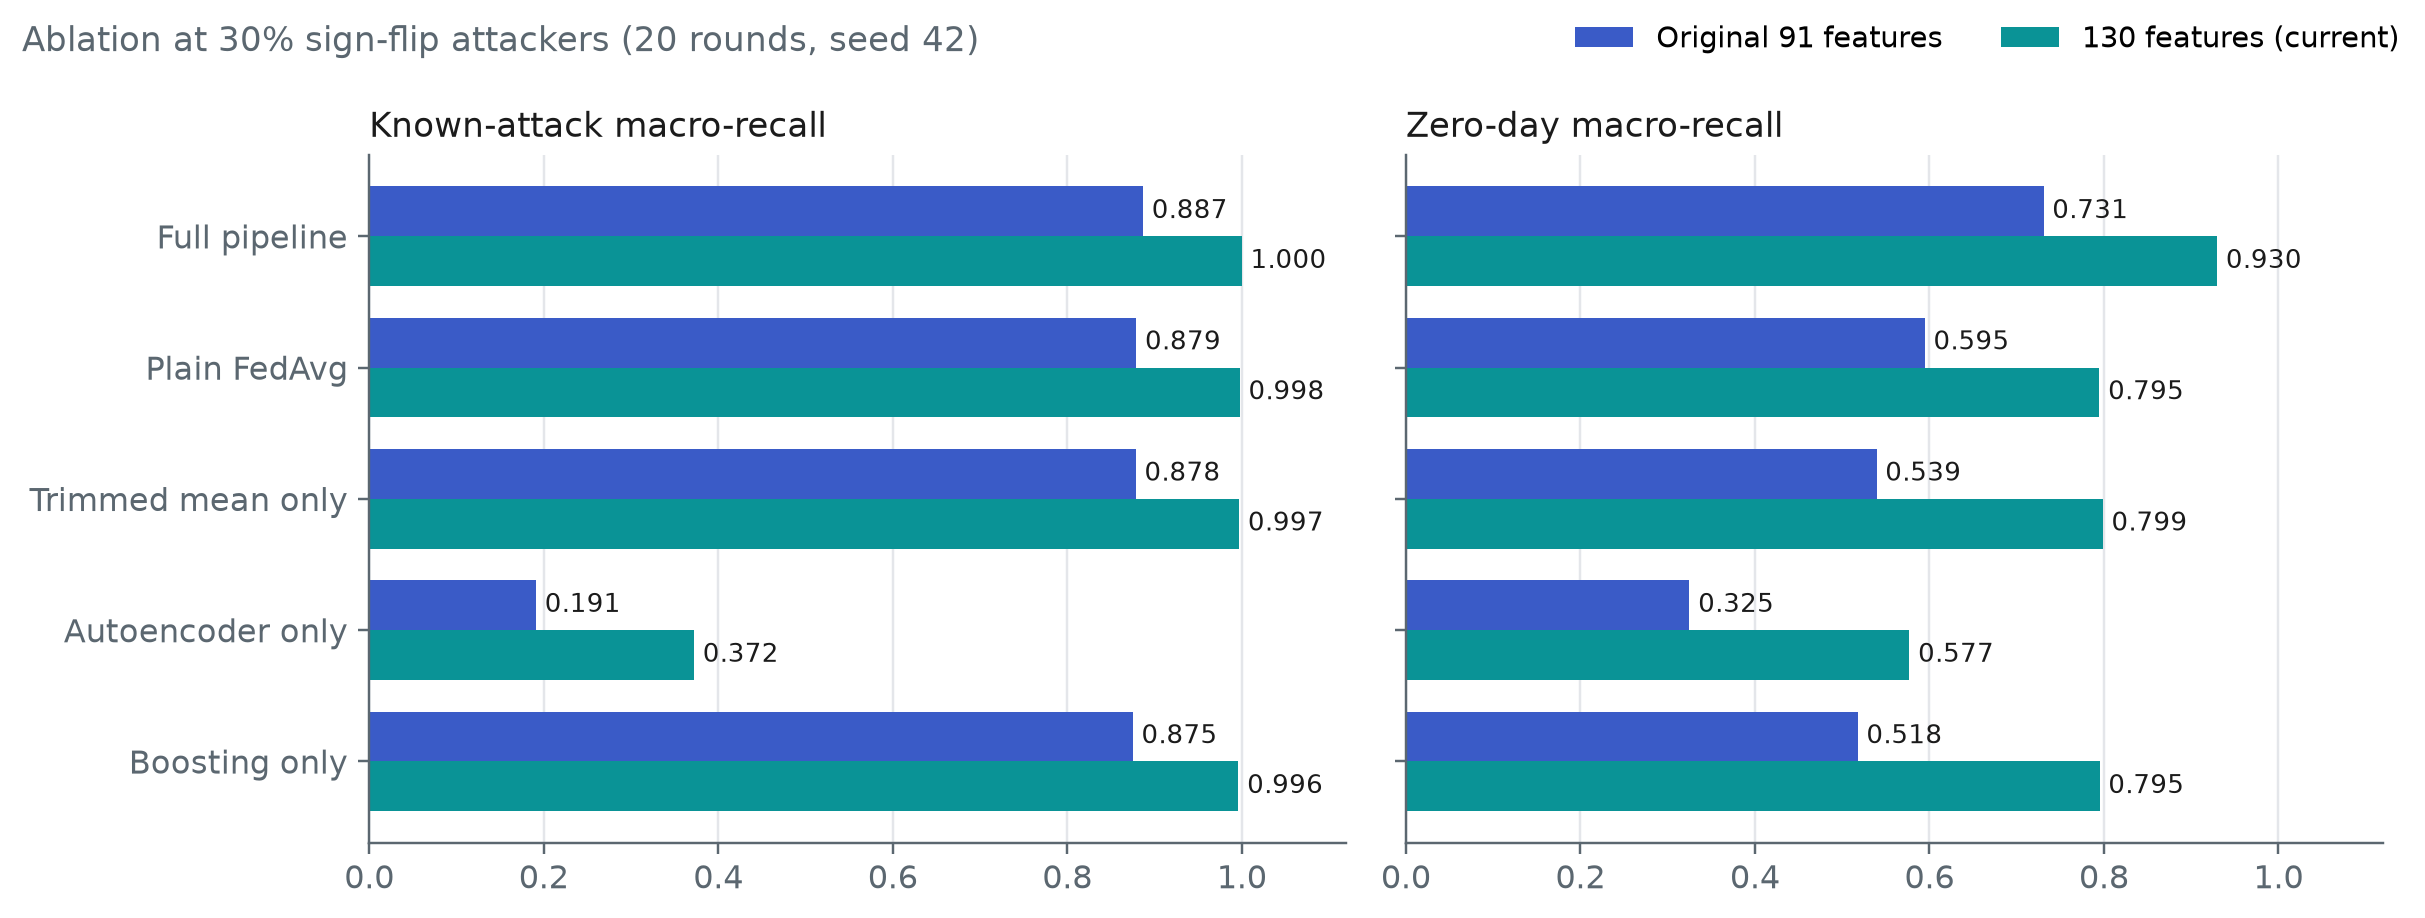
\includegraphics[width=\linewidth]{figures/ablation.png}
\caption{Ablation: known-attack and zero-day macro-recall, original vs.\ current features}
\label{fig:ablation}
\end{figure}
One trade-off is worth stating. On known attacks, boosting alone now has a higher detection F1 than the full cascade (0.998 vs.\ 0.961). The autoencoder's threshold is set to flag about 3\% of benign traffic, and that cost now outweighs the little it adds when the classifier already catches 99.6\% of known attacks. Final validation losses: full pipeline 0.028; plain FedAvg $5.0\times10^{20}$ and trimmed mean $1.3\times10^{4}$ (diverged). Communication: 15.7\,MB over 20 rounds (the autoencoder now has 9{,}834 parameters, up from 7{,}299).

\section{Poisoning resistance}
Figure~\ref{fig:poison} sweeps the share of sign-flip attackers from 0 to 50\%. Attack macro-recall stays between 0.997 and 1.000 at every fraction [0.878--0.887], and zero-day macro-recall between 0.901 and 0.943 up to 40\% [0.724--0.736]. Attackers got past the filter in 10\%, 12\% and 36\% of attacker-rounds at 20\%, 30\% and 40\% [28\%, 32\%, 24\%]: lower at the first two fractions but higher at 40\%, although the autoencoder still held there (stand-alone recall 0.691). At 50\% the coordinate-wise median reference becomes the attackers' direction again: every attacker update passes, the autoencoder collapses, and zero-day detection falls back to the classifier (0.803). This is the known limit of median-based defences~\cite{yin2018trimmed}. A repeat with seeds 43 and 44 at 20\% and 30\% gave 0.996--0.999 attack macro-recall for every seed, while stand-alone autoencoder recall varied by seed (0.56--0.74), as it did with the original features.
\begin{figure}[H]
\centering
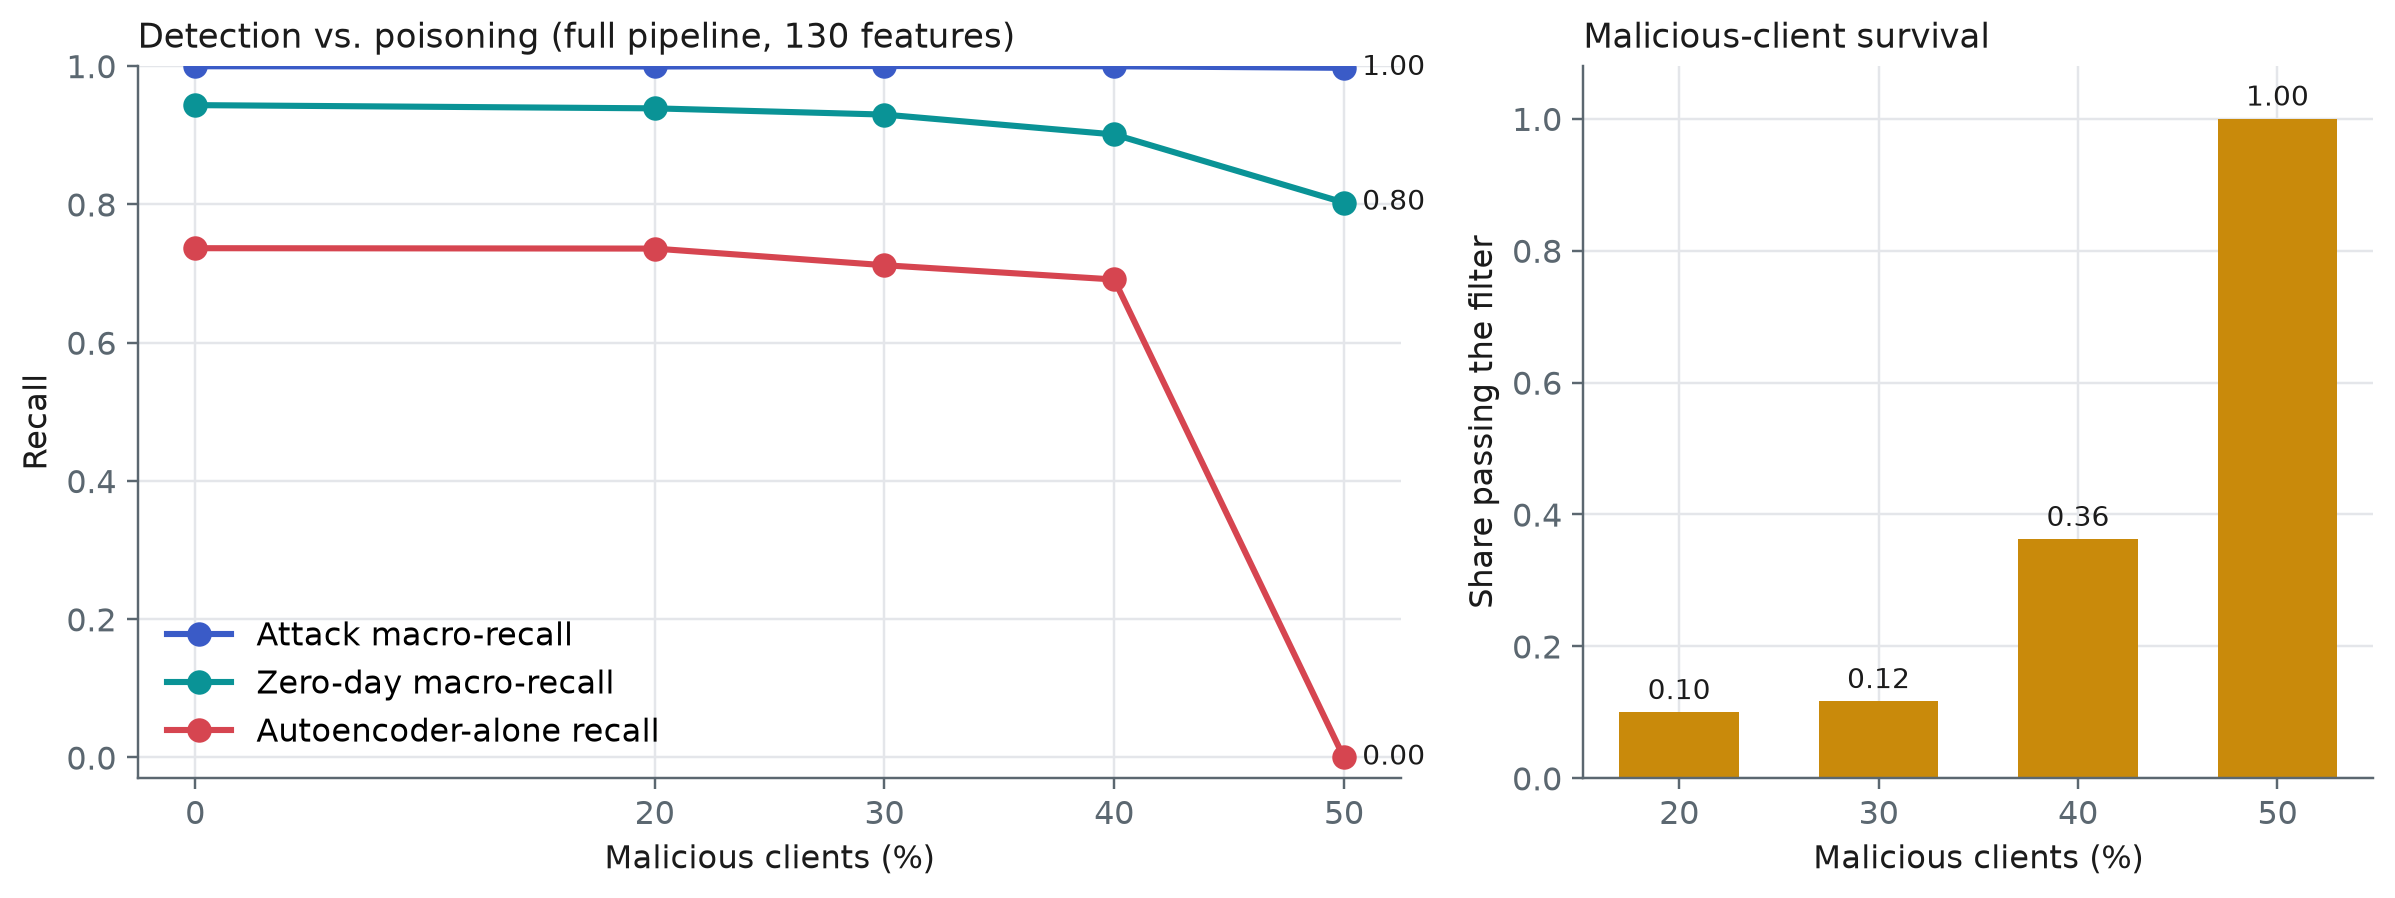
\includegraphics[width=\linewidth]{figures/poisoning_sweep.png}
\caption{Detection and malicious-client survival vs.\ share of malicious clients (130 features)}
\label{fig:poison}
\end{figure}

\section{Zero-day detection}
Each of the 14 attack classes was removed in turn from all training data (including scaler statistics) and then scored as unseen traffic (Figures~\ref{fig:zeroday} and~\ref{fig:zerodaycmp}). The cascade's average detection rose from 0.736 to \textbf{0.943}; boosting alone from 0.533 to 0.801 and the autoencoder alone from 0.493 to 0.757. The autoencoder separates unseen attacks from benign traffic far better than before (AUROC 0.968--1.000 for every class, against 0.59--0.70 for the HTTP-family attacks with the original features). The largest gains are on the attacks that were hardest before: Password 0.44$\rightarrow$0.97, Ransomware 0.54$\rightarrow$1.00, SQL\_injection 0.61$\rightarrow$1.00, XSS 0.52$\rightarrow$0.99 and DDoS\_HTTP 0.36$\rightarrow$0.88.

Two classes got worse and are reported rather than hidden. MITM fell from 0.89 to 0.69: its single ARP connection gets ordinary-looking connection features, so the autoencoder finds it less unusual. Unseen Uploading traffic now looks normal to the classifier (boosting-only 0.49$\rightarrow$0.08); the autoencoder catches most of it, so the cascade still improves (0.52$\rightarrow$0.72). The benign false-positive rate stays about 3\%, as set by the 97th-percentile threshold.
\begin{figure}[H]
\centering
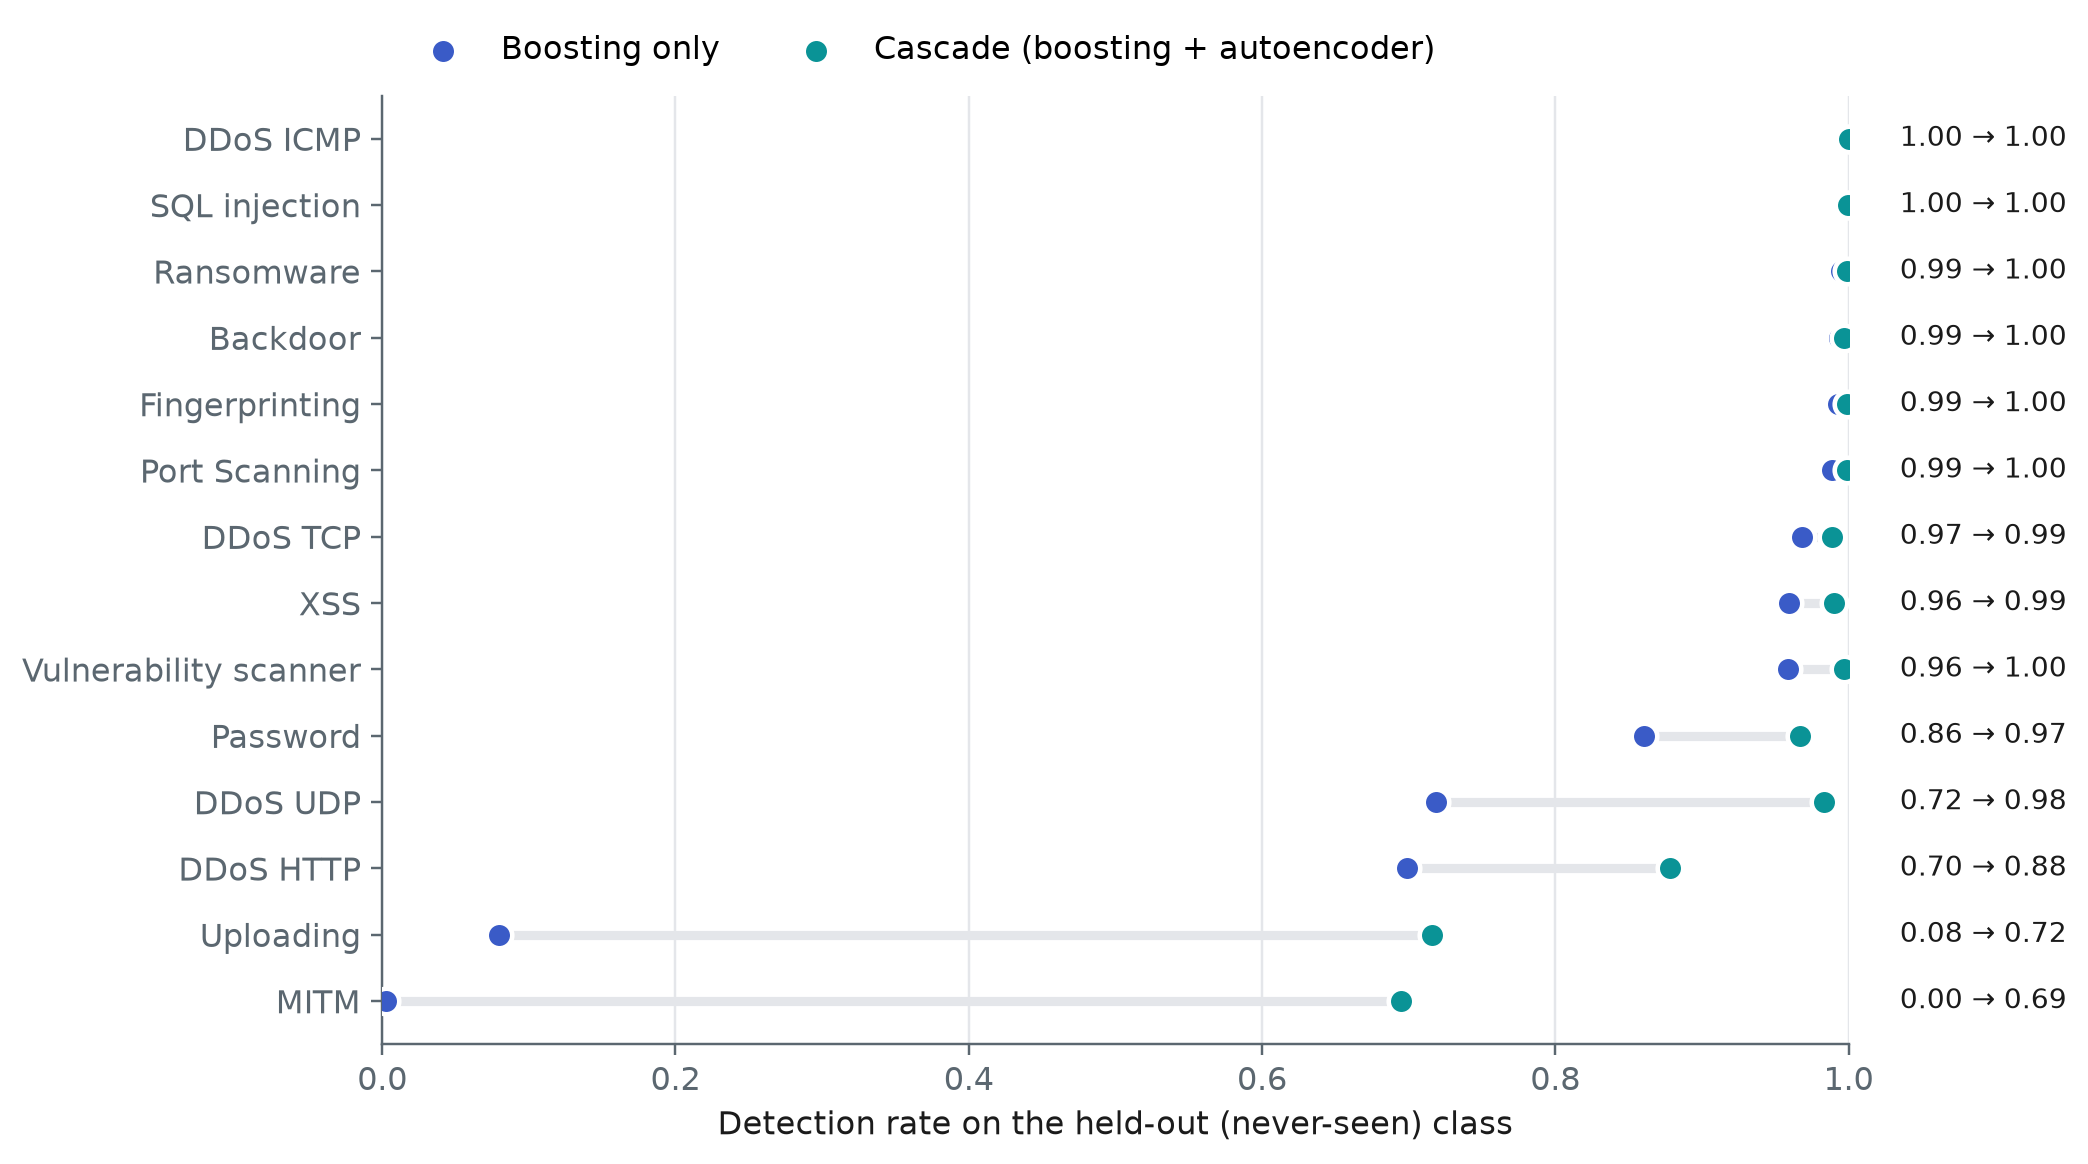
\includegraphics[width=0.88\linewidth]{figures/zero_day.png}
\caption{Zero-day detection per held-out class: boosting alone vs.\ cascade (130 features)}
\label{fig:zeroday}
\end{figure}
\begin{figure}[H]
\centering
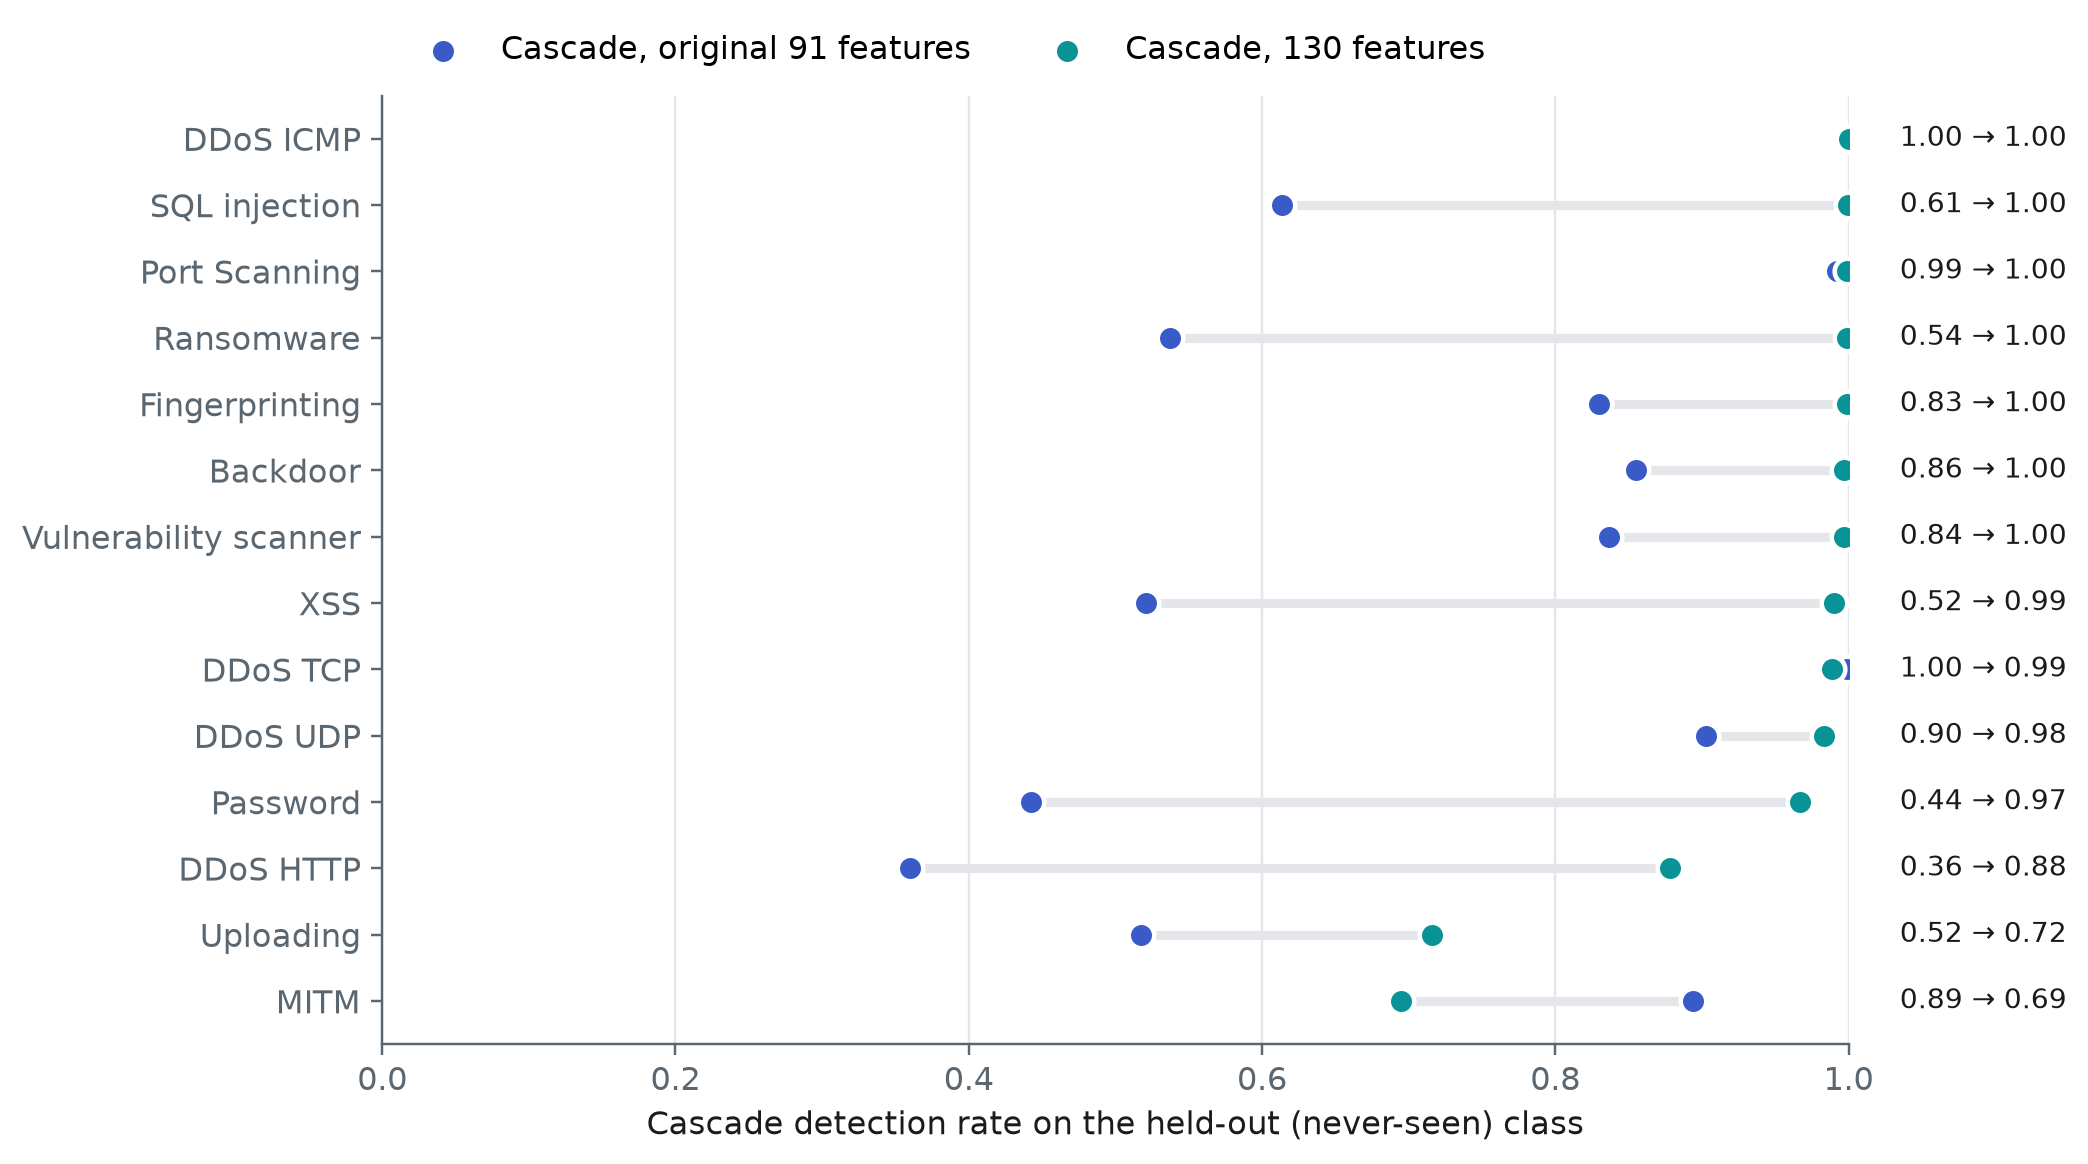
\includegraphics[width=0.88\linewidth]{figures/zero_day_compare.png}
\caption{Cascade zero-day detection per held-out class: original 91 features vs.\ 130 features}
\label{fig:zerodaycmp}
\end{figure}

\section{Real multi-process run and SDN mitigation}
\textbf{Phase A, real run.} A real Flower server and 10 separate client processes completed 20 rounds in about 4 minutes. The bootstrap classifier reached 0.997 accuracy on the calibration hold-out [0.963]. The final cascade gave \textbf{0.999} attack macro-recall [0.889] and a 0.035 benign false-positive rate [0.035] on the clients' test slices. A separate full-pipeline run scored per class gave 0.976 accuracy and 0.971 macro F1 for the cascade [0.944 / 0.931], and an autoencoder AUROC of 0.982 [0.805].

\textbf{Phase B.} Live extraction now derives the same 130 features from the capture with the same code as training: for \texttt{Backdoor\_attack.pcap}, 99.8\% of the live rows are identical to that capture's training rows. Replayed through Mininet with the new bundle, the capture was classified as \textbf{Backdoor with 0.997 confidence} by the boosting stage, 24{,}669 of its 24{,}914 packets were flagged [23{,}895], the bridge chose \emph{block}, and the rule \texttt{priority=100,ip,nw\_src=10.0.0.1 actions=drop} was confirmed in the switch's flow table. Because classification happens once features have been extracted from the whole capture, 23{,}161 replayed packets had already been forwarded when the rule appeared. The mitigation is therefore capture-level, not inline per-packet blocking.

\section{Scaling to 20 clients, repeat seeds and run timing}
\textbf{Real 20-process runs.} The project was re-hosted on a virtual machine with 24~GB of memory, which can hold one Flower server and 20 client processes (an earlier attempt on a 7.4~GB machine could not). Phase A was run with 10 and with 20 real client processes at seeds 42, 43 and 44 (20 rounds, no attackers). The seed changes the data split, the Dirichlet partition and the initialisation. Table~\ref{tab:realruns} lists every run. Over the three seeds the cascade's attack macro-recall averages 0.998 with 10 clients and 0.992 with 20 clients, and the benign false-positive rate stays between 2.8\% and 4.0\%. At seed 42, the 20-client run dips to 0.978; this run was not analysed per class, so its cause is not established. With only three seeds, no confidence intervals are claimed.

\begin{table}[H]
\centering
\renewcommand{\arraystretch}{1.2}
\begin{tabular}{|l|c|c|c|c|}
\hline
\textbf{Run} & \textbf{Phase A (s)} & \textbf{Attack macro-recall} & \textbf{False alarms} & \textbf{Classifier acc.} \\ \hline
10 clients, seed 42 & 341 & 0.999 & 3.40\% & 0.9969 \\ \hline
10 clients, seed 43 & 276 & 0.999 & 3.11\% & 0.9976 \\ \hline
10 clients, seed 44 & 262 & 0.996 & 2.84\% & 0.9968 \\ \hline
20 clients, seed 42 & 247 & 0.978 & 3.62\% & 0.9969 \\ \hline
20 clients, seed 43 & 238 & 0.999 & 2.84\% & 0.9976 \\ \hline
20 clients, seed 44 & 242 & 0.999 & 3.96\% & 0.9968 \\ \hline
\end{tabular}
\caption{Real multi-process Phase A runs (source: \texttt{results/real\_runs/summary.md})}
\label{tab:realruns}
\end{table}

Phase B on the 20-client bundle classified \texttt{Backdoor\_attack.pcap} as Backdoor with 0.997 confidence, flagged 24{,}466 of 24{,}914 packets, and the drop rule \texttt{priority=100,ip,nw\_src=10.0.0.1 actions=drop} was read back from the switch.

\textbf{The trust filter without attackers.} Even with no malicious clients, the filter excluded some clients' updates: over 20 rounds, 15, 2 and 6 client-rounds with 10 clients, and 38, 42 and 27 with 20 clients (seeds 42, 43, 44). These are honest clients whose non-IID updates look unlike the median, so the filter cannot tell unusual data from sabotage. This is the confound named in the limitations, and it is more frequent with 20 clients.

\textbf{Simulation versus real run.} An in-process simulation of 20 clients (seed 42) gave a cascade attack-detection recall of 0.9960 against 0.9996 for 10 clients, an autoencoder recall of 0.685 against 0.728, and benign false alarms of 3.72\% against 3.32\%. Three of the 20 simulated clients received no benign validation rows, so their anomaly threshold is infinite and their autoencoder never flags. The simulation uses the same client, strategy and trust-filter code as the real run, and the table above is the real-process evidence.

\textbf{Timing of one complete run.} One real run (10 client processes, warm feature cache) took 219~s in total: Phase A 210.6~s, of which federated training was 191.2~s, and Phase B 8.6~s. Tables~\ref{tab:timea} and~\ref{tab:timeb} give the stages.

\begin{table}[H]
\centering
\renewcommand{\arraystretch}{1.2}
\begin{tabular}{|l|c|}
\hline
\textbf{Phase A stage} & \textbf{Seconds} \\ \hline
Load, clean and encode the dataset & 1.9 \\ \hline
Calibration split, bootstrap classifier, client partition & 14.4 \\ \hline
Federated training & 191.2 \\ \hline
Calibrate client anomaly thresholds & 0.1 \\ \hline
Evaluate on the clients' test slices & 2.5 \\ \hline
Save the model bundle & 0.2 \\ \hline
\end{tabular}
\caption{Phase A stage timing (source: \texttt{results/journey/phase\_a\_journey.json})}
\label{tab:timea}
\end{table}

\begin{table}[H]
\centering
\renewcommand{\arraystretch}{1.2}
\begin{tabular}{|l|c|}
\hline
\textbf{Phase B stage} & \textbf{Seconds} \\ \hline
Load the model bundle & 0.08 \\ \hline
Start the SDN bridge and controller & 2.20 \\ \hline
Network, replay, classify and block (root process) & 6.33 \\ \hline
Check the switch's flow table & 0.00 \\ \hline
\end{tabular}
\caption{Phase B stage timing (source: \texttt{results/journey/phase\_b\_journey.json})}
\label{tab:timeb}
\end{table}

\section{Follow-up experiments: more seeds, an adaptive attacker, pruning and a time-ordered split}\label{sec:followups}
These experiments were run after the main results, in the virtual machine, and every table is generated from the experiments' own result files.

\textbf{More seeds.} The ablation, the poisoning sweep and the zero-day experiment were repeated at seeds 43 and 44 (Tables~\ref{tab:fu_seed_ablation}--\ref{tab:fu_seed_zeroday}). The conclusions hold in all three seeds: the full pipeline's attack macro-recall stays between 0.995 and 1.000 up to 50\% attackers; plain FedAvg and the trimmed mean alone leave the autoencoder at recall 0.000--0.026 with 30\% attackers; the trust filter fails at 50\% (attacker survival 0.97--1.00); and the cascade's mean zero-day detection is 0.943, 0.952 and 0.952. Other numbers move with the seed: the autoencoder's recall at 30\% attackers ranges from 0.565 to 0.712, attacker survival at 20\% from 0.03 to 0.23, and MITM zero-day detection from 0.695 to 0.963. The per-class zero-day columns inside the ablation and sweep tables were not repeated at seeds 43 and 44 (about 85 extra trainings per seed). Three seeds are too few for confidence intervals.

\begin{table}[H]
\centering
\small
\setlength{\tabcolsep}{3pt}
\renewcommand{\arraystretch}{1.15}
\begin{tabular}{|l|c|c|c|}
\hline
\textbf{Variant} & \textbf{Attack macro-recall} & \textbf{Autoencoder-alone recall} & \textbf{Benign FPR} \\ \hline
full\_pipeline & 1.000 / 0.999 / 0.997 & 0.712 / 0.679 / 0.565 & 0.0309 / 0.0284 / 0.0320 \\ \hline
plain\_fedavg & 0.998 / 0.997 / 0.994 & 0.002 / 0.000 / 0.000 & 0.0347 / 0.0317 / 0.0297 \\ \hline
trimmed\_mean\_only & 0.997 / 0.997 / 0.996 & 0.000 / 0.000 / 0.026 & 0.0334 / 0.0291 / 0.0337 \\ \hline
autoencoder\_only & 0.372 / 0.295 / 0.306 & 0.372 / 0.295 / 0.306 & 0.0301 / 0.0281 / 0.0325 \\ \hline
boosting\_only & 0.996 / 0.997 / 0.996 & n/a / n/a / n/a & 0.0002 / 0.0000 / 0.0005 \\ \hline
\end{tabular}
\caption{Ablation at 30\% sign-flip attackers, seeds 42 / 43 / 44 (source: results/seeds/summary.json)}
\label{tab:fu_seed_ablation}
\end{table}
\begin{table}[H]
\centering
\small
\setlength{\tabcolsep}{3pt}
\renewcommand{\arraystretch}{1.15}
\begin{tabular}{|l|c|c|c|}
\hline
\textbf{Attackers} & \textbf{Attack macro-recall} & \textbf{Autoencoder-alone recall} & \textbf{Attacker survival} \\ \hline
0\% & 1.000 / 0.999 / 0.997 & 0.737 / 0.765 / 0.612 & n/a / n/a / n/a \\ \hline
20\% & 0.999 / 0.999 / 0.996 & 0.736 / 0.739 / 0.618 & 0.10 / 0.03 / 0.23 \\ \hline
30\% & 1.000 / 0.999 / 0.997 & 0.712 / 0.679 / 0.565 & 0.12 / 0.12 / 0.27 \\ \hline
40\% & 1.000 / 0.998 / 0.997 & 0.691 / 0.620 / 0.537 & 0.36 / 0.31 / 0.44 \\ \hline
50\% & 0.997 / 0.997 / 0.995 & 0.000 / 0.000 / 0.000 & 1.00 / 0.99 / 0.97 \\ \hline
\end{tabular}
\caption{Poisoning sweep, seeds 42 / 43 / 44}
\label{tab:fu_seed_sweep}
\end{table}
\begin{table}[H]
\centering
\small
\setlength{\tabcolsep}{3pt}
\renewcommand{\arraystretch}{1.15}
\begin{tabular}{|l|c|}
\hline
\textbf{Stage} & \textbf{Mean detection rate} \\ \hline
Classifier alone & 0.801 / 0.748 / 0.791 \\ \hline
Autoencoder alone & 0.757 / 0.775 / 0.747 \\ \hline
Cascade & 0.943 / 0.952 / 0.952 \\ \hline
Cascade, DDoS\_HTTP & 0.878 / 0.846 / 0.948 \\ \hline
Cascade, MITM & 0.695 / 0.963 / 0.837 \\ \hline
Cascade, Uploading & 0.716 / 0.677 / 0.665 \\ \hline
\end{tabular}
\caption{Zero-day detection of the unseen class, mean over 14 classes, seeds 42 / 43 / 44}
\label{tab:fu_seed_zeroday}
\end{table}
\textbf{Why the 20-client run dipped.} The seed-42 run with 20 real clients scored attack macro-recall 0.978, against 0.996--0.999 elsewhere. The cause is one missed Fingerprinting test row out of four; micro recall is 0.9964 (Table~\ref{tab:fu_realrun_breakdown}). Clients without benign validation rows (infinite threshold) were still caught by the classifier.

\begin{table}[H]
\centering
\scriptsize
\setlength{\tabcolsep}{3pt}
\renewcommand{\arraystretch}{1.15}
\begin{tabular}{|l|c|c|c|c|c|}
\hline
\textbf{Run} & \textbf{Macro-recall} & \textbf{Micro recall} & \textbf{Fingerprinting test rows, recall} & \textbf{MITM test rows, recall} & \textbf{Clients with infinite threshold} \\ \hline
10 clients, seed 42 & 0.999 & 0.9992 & 3 rows, 1.00 & 3 rows, 1.00 & 0 \\ \hline
10 clients, seed 43 & 0.999 & 0.9992 & 4 rows, 1.00 & 4 rows, 1.00 & 1 \\ \hline
10 clients, seed 44 & 0.996 & 0.9960 & 4 rows, 1.00 & 5 rows, 1.00 & 1 \\ \hline
20 clients, seed 42 & 0.978 & 0.9964 & 4 rows, 0.75 & 1 rows, 1.00 & 3 \\ \hline
20 clients, seed 43 & 0.999 & 0.9992 & 2 rows, 1.00 & 3 rows, 1.00 & 2 \\ \hline
20 clients, seed 44 & 0.999 & 0.9988 & 2 rows, 1.00 & 3 rows, 1.00 & 2 \\ \hline
\end{tabular}
\caption{Where the real-run macro-recall comes from (source: results/real\_runs/<run>/, made by fl\_ids.eval.bundle\_report)}
\label{tab:fu_realrun_breakdown}
\end{table}
\textbf{Real attackers.} With sign-flip attackers in the real multi-process run, the trust filter excluded the attackers' updates in 36 of 40 (20\%) and 52 of 60 (30\%) client-rounds, and excluded no honest client (Table~\ref{tab:fu_attack_runs}, Figure~\ref{fig:trustmal03}).

\begin{table}[H]
\centering
\scriptsize
\setlength{\tabcolsep}{3pt}
\renewcommand{\arraystretch}{1.15}
\begin{tabular}{|l|c|c|c|c|c|}
\hline
\textbf{Attackers} & \textbf{Attacker clients} & \textbf{Attacker client-rounds excluded} & \textbf{Honest client-rounds excluded} & \textbf{Attack macro-recall} & \textbf{Benign FPR} \\ \hline
20\% & 0,7 & 36 of 40 & 0 of 160 & 0.998 & 0.0335 \\ \hline
30\% & 0,6,9 & 52 of 60 & 0 of 140 & 0.999 & 0.0317 \\ \hline
\end{tabular}
\caption{Real multi-process Phase A with sign-flip attackers (10 clients, 20 rounds, seed 42; source: runs/attack\_runs/)}
\label{tab:fu_attack_runs}
\end{table}
\begin{figure}[H]
\centering
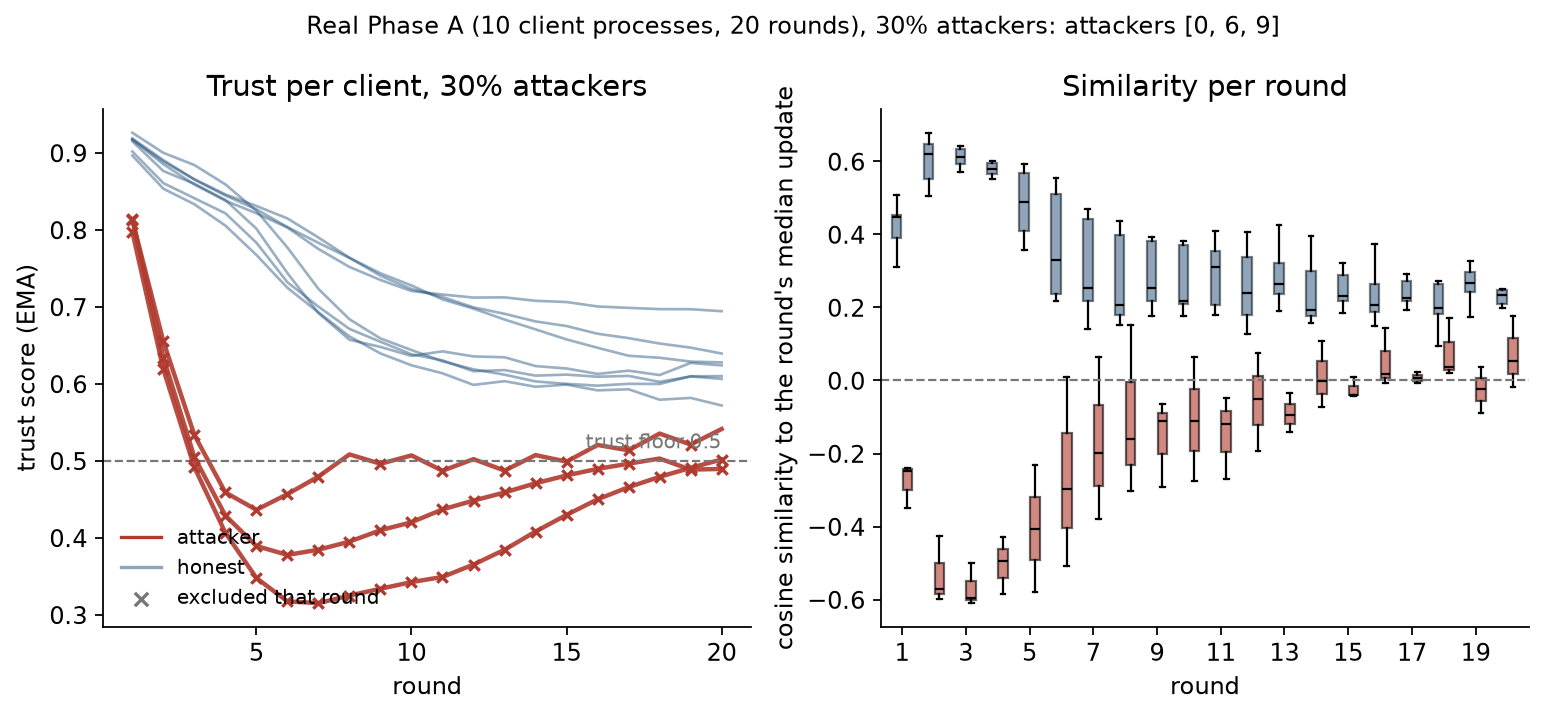
\includegraphics[width=0.98\linewidth]{figures/trust_mal03.png}
\caption{Real run with 30\% sign-flip attackers: trust score (left) and cosine similarity to the round's median update (right)}
\label{fig:trustmal03}
\end{figure}
\textbf{An adaptive attacker.} A white-box attacker that knows the filter's rule estimates the consensus from the last aggregate update, keeps a cosine similarity of 0.1 to it, and spends the rest of a norm budget (1.5 times its honest norm, under the clip) on the opposite of its honest update's orthogonal component. The filter mostly fails against it: attackers survive in 72--90\% of client-rounds instead of 10--36\% (Table~\ref{tab:fu_adaptive}). The damage is bounded: known-attack recall stays at 0.9997 or above, but the autoencoder's recall alone falls to 0.499 at 40\% attackers (0.663 for sign-flip). Zero-day detection under this attacker was not measured, and this is one adaptive strategy, not a proof for all.

\begin{table}[H]
\centering
\scriptsize
\setlength{\tabcolsep}{3pt}
\renewcommand{\arraystretch}{1.15}
\begin{tabular}{|l|c|c|c|c|c|}
\hline
\textbf{Attack} & \textbf{Attackers} & \textbf{Attack macro-recall} & \textbf{Autoencoder-alone recall} & \textbf{Attacker survival} & \textbf{Final validation loss} \\ \hline
sign\_flip & 20\% & 0.9993 & 0.730 & 0.10 & 0.026 \\ \hline
sign\_flip & 30\% & 1.0000 & 0.718 & 0.12 & 0.029 \\ \hline
sign\_flip & 40\% & 0.9997 & 0.663 & 0.36 & 0.021 \\ \hline
stealth & 20\% & 0.9997 & 0.747 & 0.90 & 0.041 \\ \hline
stealth & 30\% & 1.0000 & 0.741 & 0.72 & 0.040 \\ \hline
stealth & 40\% & 0.9997 & 0.499 & 0.82 & 0.037 \\ \hline
\end{tabular}
\caption{Adaptive (stealth) attacker vs. sign-flip, seed 42, 20 rounds (source: results/adaptive/adaptive\_attack.csv)}
\label{tab:fu_adaptive}
\end{table}
\textbf{Weight pruning (Objective 3).} The autoencoder's weight matrices were magnitude-pruned after training and during federated training (the server re-prunes every round). Pruning after training damages the backstop at once, while pruning during training keeps it up to about 70\% sparsity: autoencoder-alone recall 0.744 dense, 0.727 at 50\%, 0.688 at 70\%, then 0.467 at 80\% (Tables~\ref{tab:fu_prune_post} and~\ref{tab:fu_prune_fl}). A sparse layout needs index storage, so the size falls below the dense size only past 50\% sparsity (0.61 of the dense bytes at 70\%; computed from the non-zero counts, not transmitted). Clients still send dense updates, so this reduces the model, not the per-round communication. Single seed, no attackers.

\begin{table}[H]
\centering
\scriptsize
\setlength{\tabcolsep}{3pt}
\renewcommand{\arraystretch}{1.15}
\begin{tabular}{|l|c|c|c|c|c|c|}
\hline
\textbf{Sparsity} & \textbf{Non-zero weights} & \textbf{Sparse / dense bytes} & \textbf{Autoencoder recall} & \textbf{Autoencoder AUROC} & \textbf{Cascade macro-recall} & \textbf{Benign FPR} \\ \hline
0\% & 9600 & 1.98 & 0.742 & 0.987 & 0.999 & 0.0340 \\ \hline
50\% & 4800 & 1.00 & 0.273 & 0.742 & 0.998 & 0.0287 \\ \hline
70\% & 2880 & 0.61 & 0.168 & 0.596 & 0.998 & 0.0292 \\ \hline
80\% & 1920 & 0.41 & 0.145 & 0.559 & 0.996 & 0.0334 \\ \hline
90\% & 960 & 0.22 & 0.144 & 0.594 & 0.996 & 0.0323 \\ \hline
95\% & 480 & 0.12 & 0.147 & 0.593 & 0.996 & 0.0366 \\ \hline
98\% & 192 & 0.06 & 0.147 & 0.593 & 0.996 & 0.0366 \\ \hline
\end{tabular}
\caption{Post-training magnitude pruning of the 10-client autoencoder, thresholds recalibrated (source: results/pruning/c10\_s42/pruning.csv)}
\label{tab:fu_prune_post}
\end{table}
\begin{table}[H]
\centering
\scriptsize
\setlength{\tabcolsep}{3pt}
\renewcommand{\arraystretch}{1.15}
\begin{tabular}{|l|c|c|c|c|c|c|}
\hline
\textbf{Sparsity} & \textbf{Non-zero weights} & \textbf{Sparse / dense bytes} & \textbf{Autoencoder-alone recall} & \textbf{Cascade macro-recall} & \textbf{Benign FPR} & \textbf{Final validation loss} \\ \hline
0\% & 9600 & 1.98 & 0.744 & 1.000 & 0.0320 & 0.034 \\ \hline
50\% & 4800 & 1.00 & 0.727 & 1.000 & 0.0323 & 0.040 \\ \hline
70\% & 2880 & 0.61 & 0.688 & 1.000 & 0.0298 & 0.049 \\ \hline
80\% & 1920 & 0.41 & 0.467 & 0.999 & 0.0312 & 0.080 \\ \hline
90\% & 960 & 0.22 & 0.176 & 0.998 & 0.0289 & 0.207 \\ \hline
\end{tabular}
\caption{Pruning during federated training (server re-prunes each round, linear ramp over the first 10 rounds), seed 42, no attackers (source: results/pruning/pruning\_during\_fl.csv)}
\label{tab:fu_prune_fl}
\end{table}
\textbf{Clipping.} Without the per-client z-score clip the benign validation loss stays near 50; with it, it falls from 0.2047 to 0.03369 (Table~\ref{tab:fu_clip}, Figure~\ref{fig:clipval}).

\begin{table}[H]
\centering
\scriptsize
\setlength{\tabcolsep}{3pt}
\renewcommand{\arraystretch}{1.15}
\begin{tabular}{|l|c|c|c|c|}
\hline
\textbf{Normalisation} & \textbf{Round 1} & \textbf{Round 5} & \textbf{Round 10} & \textbf{Round 20} \\ \hline
clip 10 & 0.2047 & 0.04336 & 0.03999 & 0.03369 \\ \hline
no clip & 50.63 & 50.15 & 50 & 49.86 \\ \hline
\end{tabular}
\caption{Benign validation loss with and without the per-client z-score clip (source: results/clip/clip\_comparison.csv)}
\label{tab:fu_clip}
\end{table}
\begin{figure}[H]
\centering
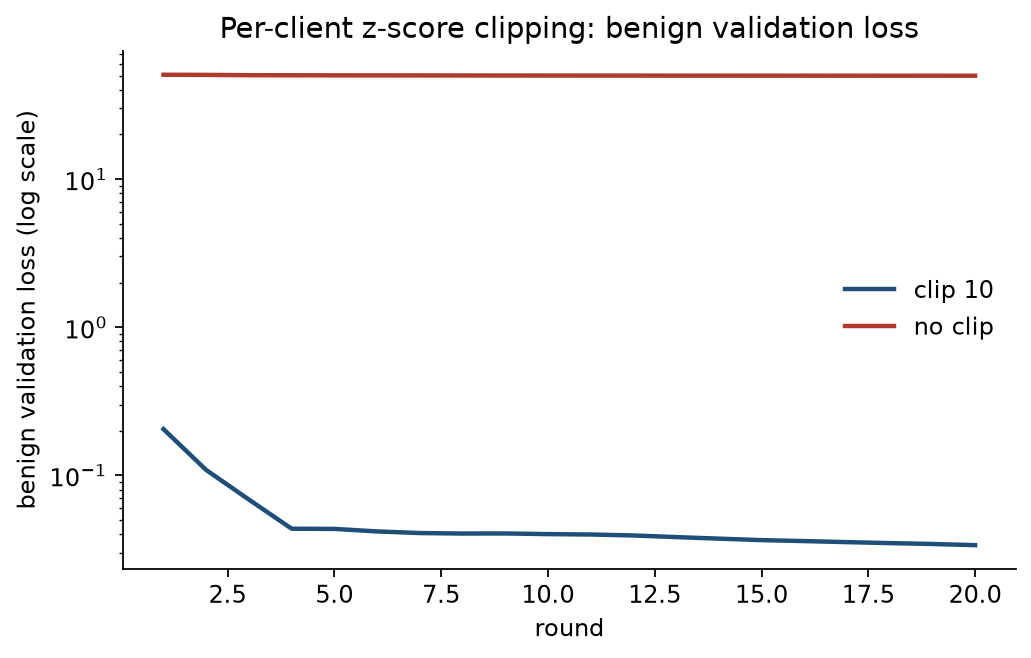
\includegraphics[width=0.7\linewidth]{figures/clip_val_loss.png}
\caption{Benign validation loss with and without the per-client z-score clip}
\label{fig:clipval}
\end{figure}
\textbf{A time-ordered split.} Each class's earliest 80\% of connections were used for training and its latest 20\% for testing (the CSV is in capture order within a class, but its timestamps carry no date, so this orders by row position). Accuracy is 0.994 against 0.997 for the connection-grouped split (Table~\ref{tab:fu_temporal_summary}). Macro F1 falls from 0.983 to 0.913, mostly because MITM is a single connection, so it falls entirely in the test side and enters the mean with recall 0; without it the figure is about 0.978. The real losses are Backdoor (0.989 to 0.947--0.962) and DDoS\_HTTP (0.980 to 0.912--0.925).

\begin{table}[H]
\centering
\small
\setlength{\tabcolsep}{3pt}
\renewcommand{\arraystretch}{1.15}
\begin{tabular}{|l|c|c|}
\hline
\textbf{Split} & \textbf{Accuracy} & \textbf{Macro F1} \\ \hline
Time-ordered, seeds 42 / 43 / 44 & 0.9942 / 0.9943 / 0.9941 & 0.9133 / 0.9122 / 0.9129 \\ \hline
Connection-grouped, seed 42 & 0.9972 & 0.9828 \\ \hline
\end{tabular}
\caption{Per-class time-ordered split vs. connection-grouped split (source: experiments/accuracy/results/full\_temporal\_bal\_s*.json)}
\label{tab:fu_temporal_summary}
\end{table}
\textbf{The placeholder leak, measured.} Before the fix, the four affected raw columns separate attack from normal with AUROC 0.9998--1.0. On the current 130-feature matrix the strongest single feature is the flow's reset count (0.879), followed by its packet count (0.866) and the service port (0.835); these are connection summaries rather than spelling artifacts (Table~\ref{tab:fu_leak}, Figure~\ref{fig:leakauroc}).

\begin{table}[H]
\centering
\small
\setlength{\tabcolsep}{3pt}
\renewcommand{\arraystretch}{1.15}
\begin{tabular}{|l|c|c|}
\hline
\textbf{Feature} & \textbf{AUROC} & \textbf{State} \\ \hline
mqtt.topic == 0.0 & 1.0000 & raw, before the fix \\ \hline
mqtt.conack.flags == 0.0 & 1.0000 & raw, before the fix \\ \hline
mqtt.protoname == 0.0 & 1.0000 & raw, before the fix \\ \hline
dns.qry.name.len == 0.0 & 0.9998 & raw, before the fix \\ \hline
f\_rst & 0.8789 & 130-feature matrix, after \\ \hline
f\_npkts & 0.8657 & 130-feature matrix, after \\ \hline
svc\_port & 0.8350 & 130-feature matrix, after \\ \hline
f\_fin & 0.8039 & 130-feature matrix, after \\ \hline
f\_pl\_nonzero & 0.7328 & 130-feature matrix, after \\ \hline
f\_syn & 0.7108 & 130-feature matrix, after \\ \hline
\end{tabular}
\caption{Single-feature AUROC, attack vs. normal (source: results/leak/single\_feature\_auroc.json; after: 300,000-row sample)}
\label{tab:fu_leak}
\end{table}
\begin{figure}[H]
\centering
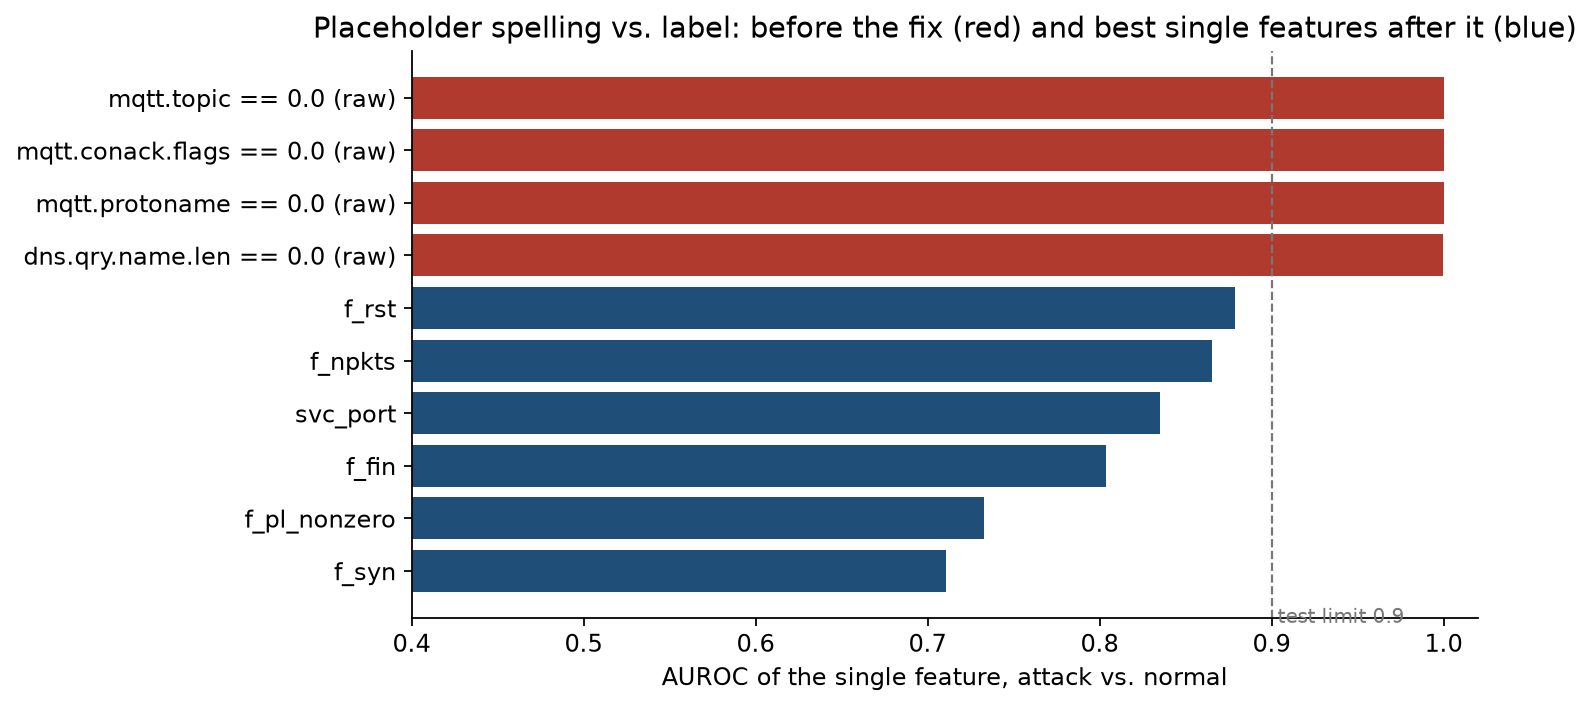
\includegraphics[width=0.8\linewidth]{figures/leak_auroc.png}
\caption{Single-feature AUROC before the placeholder fix (red) and best single features after it (blue)}
\label{fig:leakauroc}
\end{figure}
\begin{figure}[H]
\centering
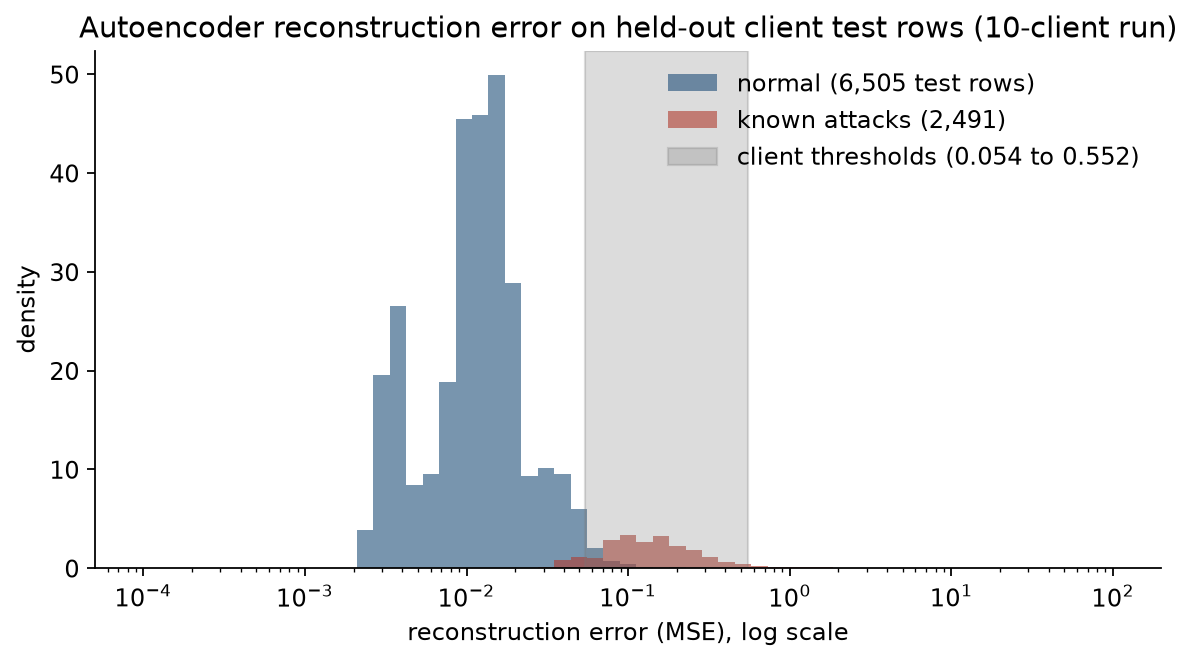
\includegraphics[width=0.8\linewidth]{figures/reconstruction_error.png}
\caption{Autoencoder reconstruction error on held-out client test rows (10-client run); grey band: range of the clients' thresholds}
\label{fig:reconerr}
\end{figure}
\begin{figure}[H]
\centering
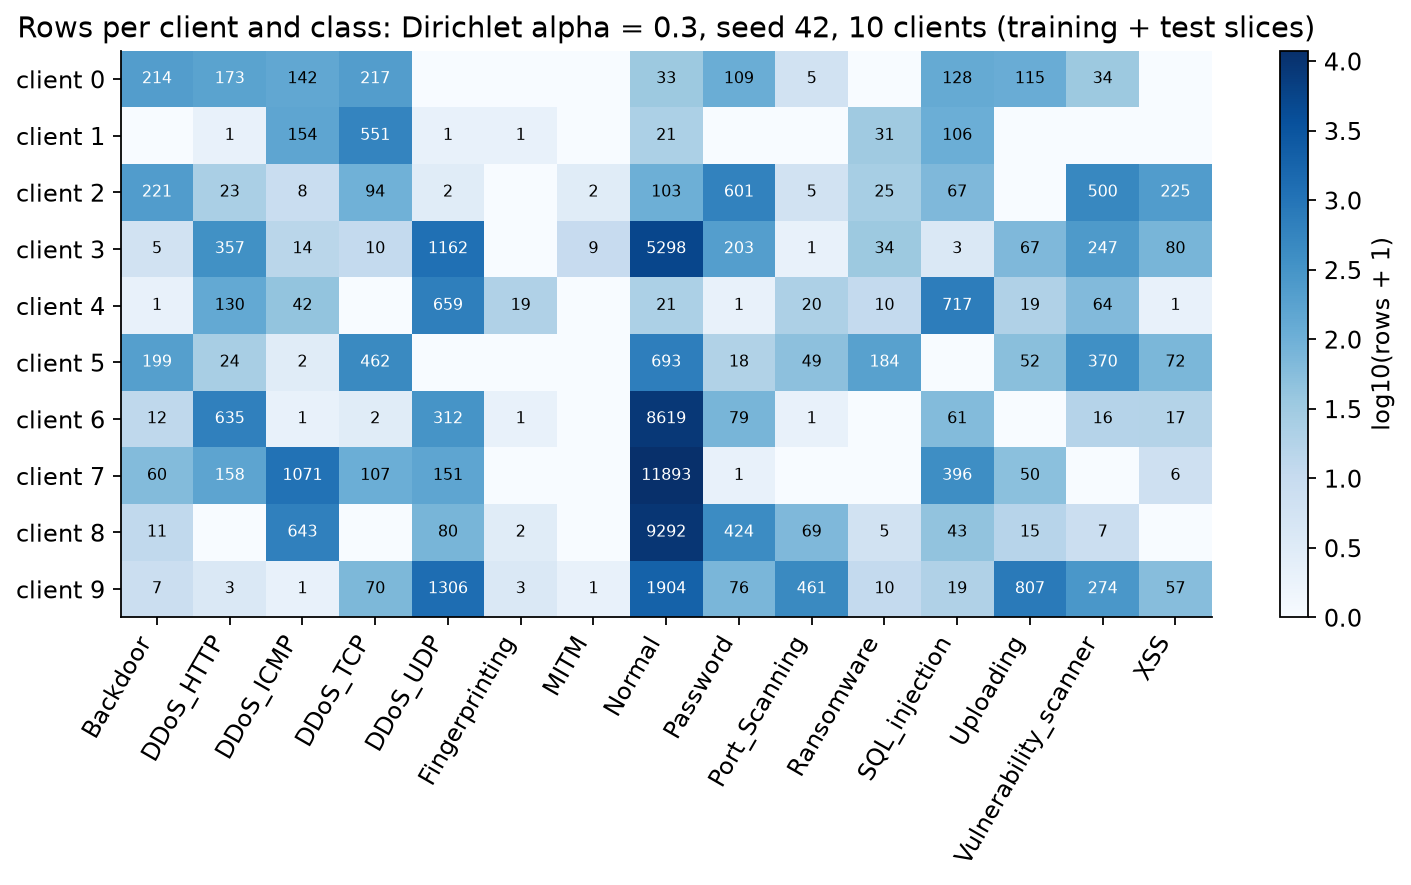
\includegraphics[width=0.98\linewidth]{figures/partition_heatmap.png}
\caption{Rows per client and class for the 10-client run (Dirichlet $\alpha=0.3$, seed 42)}
\label{fig:partheat}
\end{figure}
\begin{figure}[H]
\centering
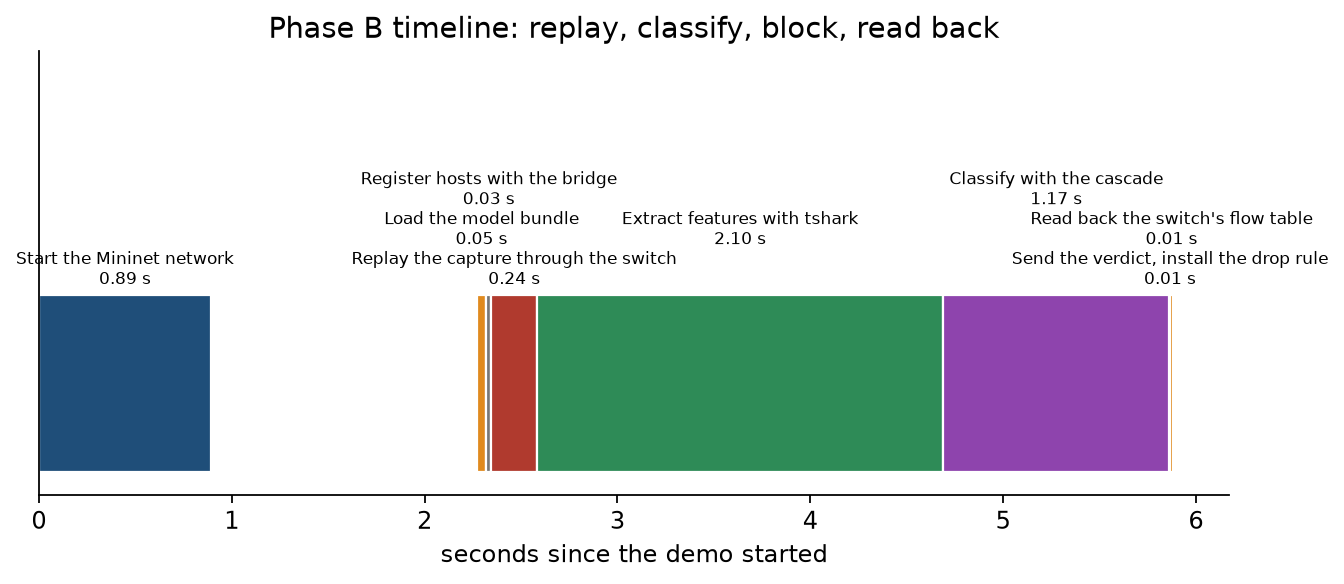
\includegraphics[width=0.9\linewidth]{figures/phase_b_timeline.png}
\caption{Phase B timeline for one replay of the Backdoor capture}
\label{fig:pbtimeline}
\end{figure}

\section{Boosting vs.\ a deep-learning classifier}
On the same 500{,}000-row sample, LightGBM (base features) reached 0.887 macro F1 and a dense MLP of comparable effort (8{,}271 parameters, 15 epochs) reached 0.622. The gap was largest on the application-layer attacks (XSS 0.761 vs.\ 0.072 recall; SQL\_injection 0.767 vs.\ 0.183). This supports the boosting-first design. It is a comparison against a modest baseline, not a claim that deep learning cannot work here.

\chapter{Conclusion and Future Work}

\section*{Conclusion}
FL-IDS shows that the five parts of the system work together on real IoT/IIoT traffic: a boosting classifier, a federated autoencoder backstop, a cosine-similarity trust filter, Flower-based federated learning, and SDN mitigation. Each part has a measured contribution. All planned phases are complete (Table~\ref{tab:workplan}); what remains is the research paper.

\begin{itemize}
  \item \textbf{Accuracy target met.} With service-port, payload-content and flow features and square-root class weights, the LightGBM classifier reaches \textbf{99.7\% accuracy and 0.983--0.985 macro F1} when trained on 1.43 million packets and tested on 397 thousand packets from connections that never appear in training (a flow-grouped 80/20 split of all 1.99 million unique packets). That is up from 96.4\% and 0.889 with the original features. The result holds across three seeds, and it holds when the classifier is trained on only the 5\% server calibration set (99.7\% / 0.979).
  \item \textbf{The whole federated system improves with the new features.} A real run with ten client processes reaches 0.999 attack macro-recall (was 0.889), and the cascade detects never-seen attack classes at 0.943 macro-recall (was 0.736), against 0.801 for the classifier alone. The backstop's value is now clearest on unseen attacks: on known attacks the classifier alone has the higher detection F1 (0.998 vs.\ 0.961).
  \item \textbf{The trust filter keeps federated training usable under poisoning.} Attack detection stays at 0.997--1.000 and zero-day detection at 0.90--0.94 up to 40\% malicious clients, while plain FedAvg's autoencoder diverges at 30\%. The filter fails at 50\%, as expected for median-based defences.
  \item \textbf{Detection drives enforcement.} Phase B derives the same features live (99.8\% of live rows match training rows exactly); a replayed Backdoor capture was classified with 0.997 confidence and produced a drop rule, confirmed from the switch's flow table.
  \item \textbf{Data quality.} The released Edge-IIoTset CSV contains a placeholder label leak (one feature with an AUROC of 1.0), first reported by Galal~\cite{galal2026provenance}, and column-shifted MITM rows, which we found and repaired. Results trained directly on it are likely inflated.
\end{itemize}

\section*{Limitations}
The service-port feature benefits from the testbed's lack of benign HTTP traffic. Two attack classes are detected less well as zero-day attacks with the new features (MITM, and Uploading for the classifier alone), and attacker survival at 40\% rose from 24\% to 36\% in a single-seed run. Flow features are computed per 120-second flow record, so classification is not per-packet. Mitigation in Phase B is capture-level rather than inline. Two attack models were tested against the trust filter (sign-flip, and a white-box stealth attacker that the filter mostly misses), and the stealth, pruning and clipping experiments use one seed. At full scale the false-alarm rate is 2.5\% to 16.3\% of normal packets but only 0.34\% to 1.04\% of normal connections, because a few very long connections dominate the packet count; the trust filter and the autoencoder backstop are weaker than at 60{,}000 rows; MITM, a single connection, is scored only by the zero-day experiment and the live replay; and two of the 14 captures are classified as the wrong type in the live replay (both are still blocked). The federated system now trains on all usable rows (Section~\ref{sec:fullpool}), but its bootstrap classifier starts from the 5\% server set; the standalone classifier trained on 1.43 million rows (Table~\ref{tab:datascale}). The classifier update ships a small number of confirmed alert rows to the server, which relaxes strict data locality.

\section*{Future Work}
\begin{enumerate}
  \item Make mitigation streaming: classify flows incrementally (for example after the first $n$ packets) so a rule can be installed while an attack is still running.
  \item Defend against the white-box stealth attacker (Section~\ref{sec:followups}), which the filter mostly misses, for example with a small trusted root dataset as in FLTrust~\cite{cao2021fltrust}; measure zero-day detection under it; and test other adaptive strategies and attackers above 50\%.
  \item Add more seeds (now three) and confidence intervals to the ablation, poisoning sweep and zero-day experiments, and repeat the zero-day columns inside the first two at the extra seeds.
  \item Find out why the trust filter excludes fewer attackers at full scale, and repeat the stealth-attacker, pruning and clipping experiments at full scale over more seeds.
  \item Validate on a second dataset that contains benign web traffic, to measure how much the service-port feature depends on the testbed.
  \item Reduce the per-round communication as well: weight pruning (Objective 3, Section~\ref{sec:followups}) shrinks the model, with autoencoder recall 0.744 dense and 0.688 at 70\% sparsity, but clients still send dense updates. Sparse updates, and zero-day detection of pruned models, remain to be done.
  \item Federate the classifier itself (for example with histogram-based federated boosting) so the calibration set no longer needs to be held centrally.
  \item Deploy on physical edge hardware and a hardware OpenFlow switch.
\end{enumerate}


\clearpage
% ----- References -----
\renewcommand{\bibname}{REFERENCES} % report class titles thebibliography itself
\addcontentsline{toc}{chapter}{REFERENCES}
\begin{thebibliography}{99}
\bibitem{ferrag2022edge} M. A. Ferrag, O. Friha, D. Hamouda, L. Maglaras and H. Janicke, ``Edge-IIoTset: A New Comprehensive Realistic Cyber Security Dataset of IoT and IIoT Applications for Centralized and Federated Learning'', \textit{IEEE Access}, vol. 10, pp. 40281--40306, 2022, doi: 10.1109/ACCESS.2022.3165809.
\bibitem{mothukuri2022fl} V. Mothukuri, P. Khare, R. M. Parizi, S. Pouriyeh \textit{et al.}, ``Federated-Learning-Based Anomaly Detection for IoT Security Attacks'', \textit{IEEE Internet of Things Journal}, vol. 9, no. 4, 2022.
\bibitem{li2021deepfed} B. Li, Y. Wu, J. Song, R. Lu, T. Li and L. Zhao, ``DeepFed: Federated Deep Learning for Intrusion Detection in Industrial Cyber--Physical Systems'', \textit{IEEE Transactions on Industrial Informatics}, vol. 17, no. 8, Aug. 2021.
\bibitem{hernandez2025fliids} J. L. Hernandez-Ramos, G. Karopoulos, E. Chatzoglou, V. Kouliaridis, E. Marmol, A. Gonzalez-Vidal and G. Kambourakis, ``Intrusion Detection Based on Federated Learning: A Systematic Review'', \textit{ACM Computing Surveys}, vol. 57, no. 12, 2025, doi: 10.1145/3731596.
\bibitem{cao2021fltrust} X. Cao, M. Fang, J. Liu and N. Z. Gong, ``FLTrust: Byzantine-robust Federated Learning via Trust Bootstrapping'', in \textit{Proc. Network and Distributed System Security Symposium (NDSS)}, 2021.
\bibitem{xu2022signguard} J. Xu, S.-L. Huang, L. Song and T. Lan, ``Byzantine-robust Federated Learning through Collaborative Malicious Gradient Filtering'' (SignGuard), in \textit{Proc. IEEE International Conference on Distributed Computing Systems (ICDCS)}, 2022.
\bibitem{zhang2023lgbmae} H. Zhang, L. Ge, G. Zhang, J. Fan, D. Li and C. Xu, ``A two-stage intrusion detection method based on light gradient boosting machine and autoencoder'', \textit{Mathematical Biosciences and Engineering}, vol. 20, no. 4, 2023, doi: 10.3934/mbe.2023301.
\bibitem{elhouda2023mitfed} Z. Abou El Houda, A. S. Hafid and L. Khoukhi, ``MiTFed: A Privacy Preserving Collaborative Network Attack Mitigation Framework Based on Federated Learning Using SDN and Blockchain'', \textit{IEEE Transactions on Network Science and Engineering}, vol. 10, no. 4, pp. 1985--2001, 2023.
\bibitem{mcmahan2017fedavg} B. McMahan, E. Moore, D. Ramage, S. Hampson and B. A. y Arcas, ``Communication-Efficient Learning of Deep Networks from Decentralized Data'', in \textit{Proc. International Conference on Artificial Intelligence and Statistics (AISTATS)}, 2017.
\bibitem{yin2018trimmed} D. Yin, Y. Chen, K. Ramchandran and P. Bartlett, ``Byzantine-Robust Distributed Learning: Towards Optimal Statistical Rates'', in \textit{Proc. International Conference on Machine Learning (ICML)}, 2018.
\bibitem{ke2017lightgbm} G. Ke, Q. Meng, T. Finley, T. Wang, W. Chen, W. Ma, Q. Ye and T.-Y. Liu, ``LightGBM: A Highly Efficient Gradient Boosting Decision Tree'', in \textit{Advances in Neural Information Processing Systems (NeurIPS)}, 2017.
\bibitem{hsu2019noniid} T.-M. H. Hsu, H. Qi and M. Brown, ``Measuring the Effects of Non-Identical Data Distribution for Federated Visual Classification'', arXiv:1909.06335, 2019.
\bibitem{galal2026provenance} M. M. Galal, ``Provenance, Not Behaviour: A Serialisation Artifact in Edge-IIoTset and a Leakage-Free Benchmark for Precision-Agriculture Intrusion Detection'', arXiv:2608.15761 (preprint), Aug. 2026.
\bibitem{sharafaldin2018cicids} I. Sharafaldin, A. H. Lashkari and A. A. Ghorbani, ``Toward Generating a New Intrusion Detection Dataset and Intrusion Traffic Characterization'', in \textit{Proc. International Conference on Information Systems Security and Privacy (ICISSP)}, 2018.
\end{thebibliography}
\clearpage

% ----- Appendices -----
\appendix
\renewcommand{\thechapter}{\Alph{chapter}}
\renewcommand{\thesection}{\Roman{section}}
\section {Appendix A: Snapshots}
\begin{figure}[H]
\centering
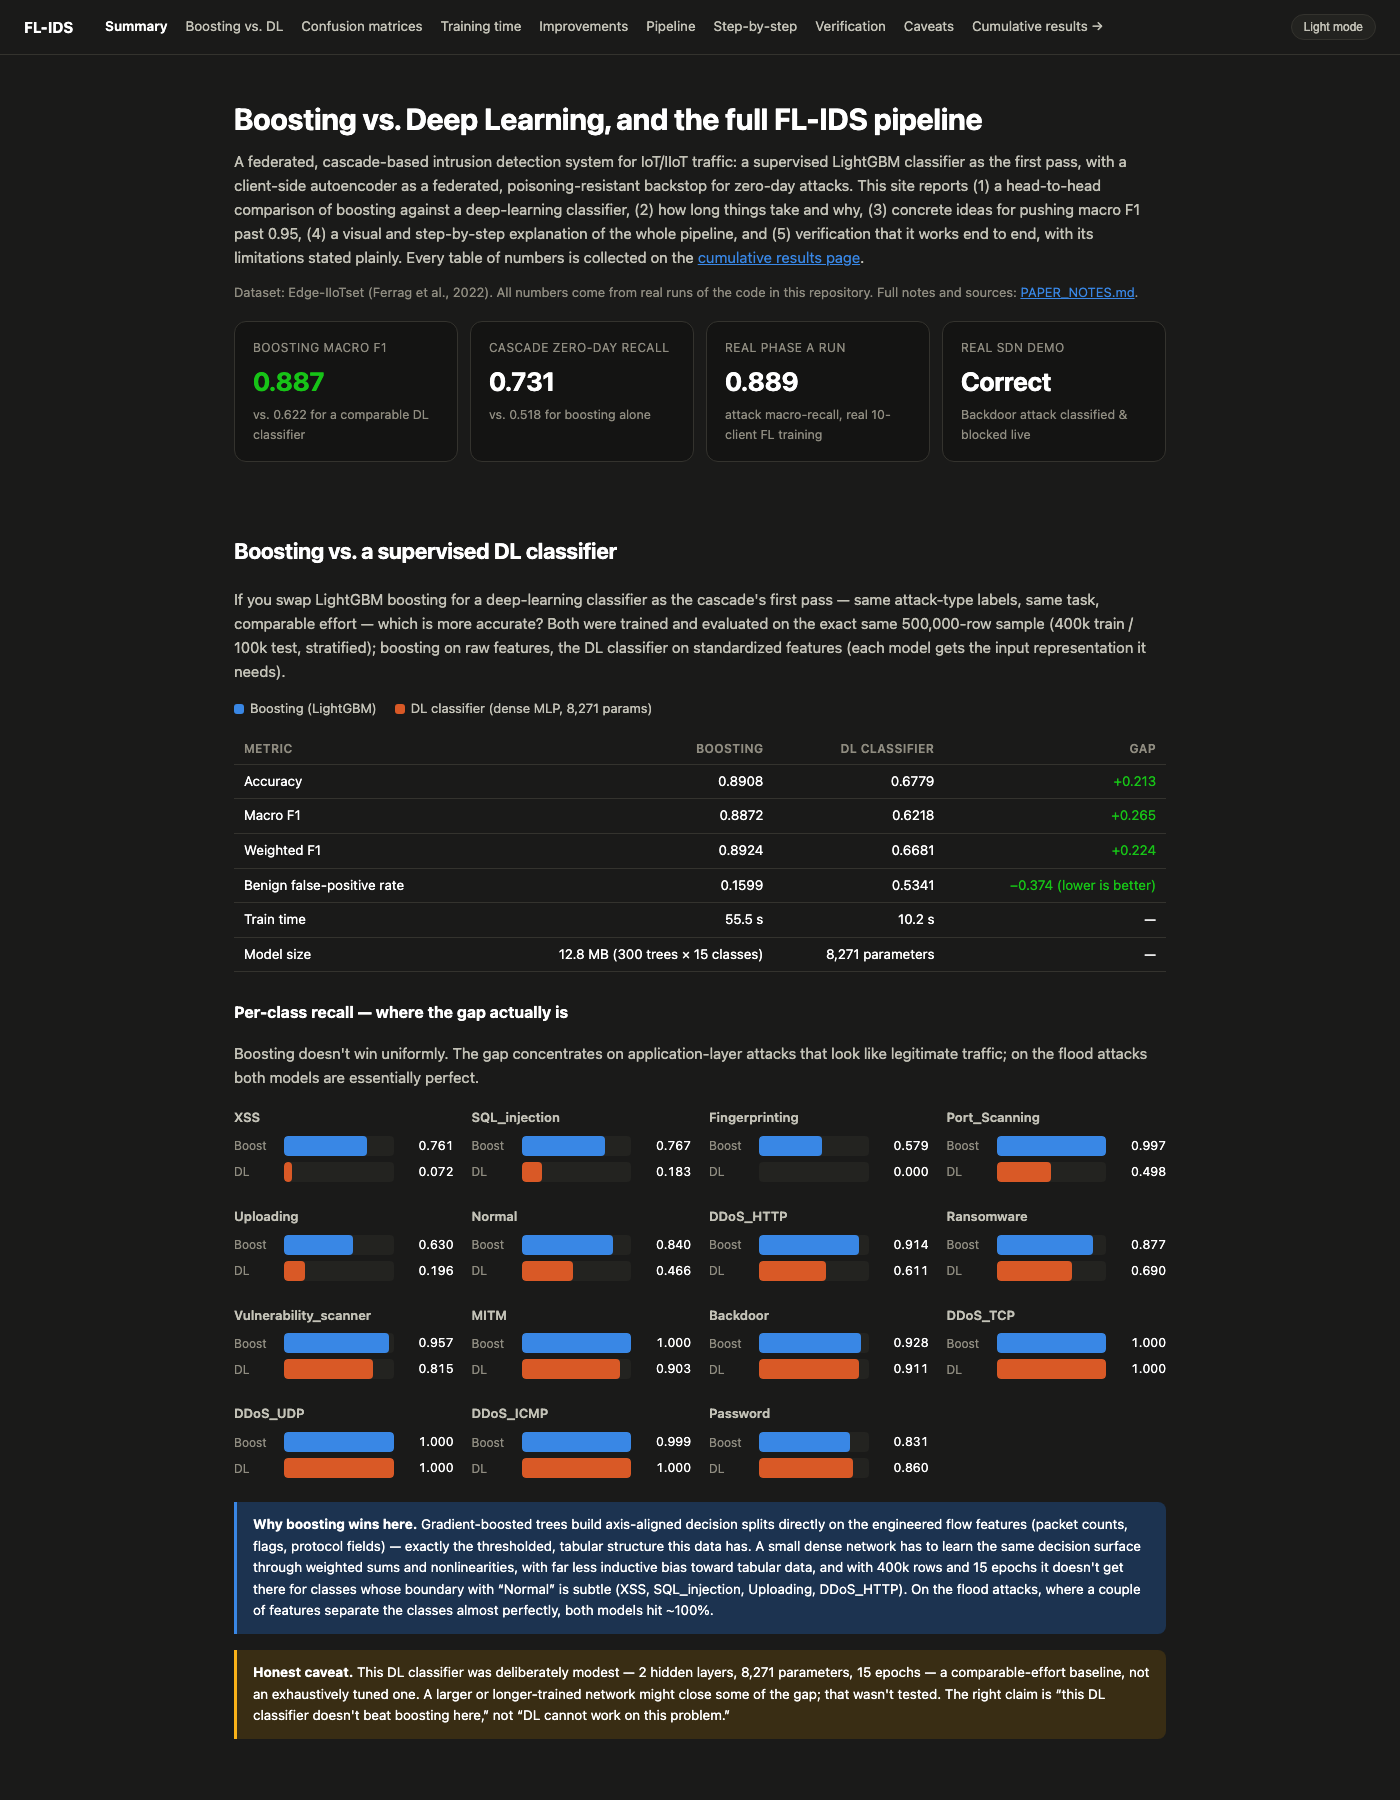
\includegraphics[width=0.9\linewidth]{figures/website.png}
\caption{Project results website (\url{https://aronnnn1.github.io/FL-IDS/})}
\end{figure}
\noindent\textbf{Phase B result} (\texttt{runs/phase\_b/phase\_b\_result.json}, excerpt):
\begin{verbatim}
"classification": "Backdoor", "confidence": 0.9974,
"stage": "boosting", "num_packets": 24914,
"num_non_benign": 23895
"mitigation": {"action": "block", "applied": true,
               "ip_address": "10.0.0.1"}
flow table:
 priority=100,ip,nw_src=10.0.0.1 actions=drop
 priority=0 actions=NORMAL   (n_packets=23586)
"check": {"action": "block", "consistent": true}
\end{verbatim}
\noindent\textbf{Automated test suite:}
\begin{verbatim}
224 passed, 2 skipped, 2 warnings in 374.08s (0:06:14)
\end{verbatim}
\clearpage
\section {Appendix B: Details of list of publications related to this project}
{\large Author Names: } Aaron B Ajay, Aaryan Prakash, Amal Roy, Amogh Krishna JS, Syed Akram \\
{\large Paper Title: } FL-IDS: Federated Learning-Based Intrusion Detection System for IoT/IIoT (working title) \\
{\large Name of the Conference or Journal:} Paper in preparation (draft in progress) \\
{\large Place of the conference:} -- \\
{\large Date of Conference:} --
\clearpage
\section {Appendix C: Details of Patent}
No patent has been filed for this work.
\clearpage
\section {Appendix D: Details of Funding}
This project did not receive external funding.
\clearpage
\section {Appendix E:POs and PSOs Mapped}
\begin{table}[h!]
\centering
\small
\renewcommand{\arraystretch}{1.05} % Row height
\setlength{\tabcolsep}{6pt}       % Column spacing
\begin{tabular}{|>{\raggedright\arraybackslash}p{3.6cm}|c|p{7.9cm}|}
\hline
\textbf{PROGRAMME OUTCOMES} & \textbf{Level (1/2/3)} & \textbf{Justification if addressed} \\
\hline
PO1 (Engineering knowledge) & 3 & Applies mathematics (cosine similarity, robust statistics, gradient boosting) and networking and machine-learning fundamentals to detecting attacks in IoT/IIoT traffic. \\
\hline
PO2 (Problem analysis) & 3 & Reviews the literature to identify gaps, and analyses why accuracy was stuck (content-free packets, ambiguity ceiling) and why aggregation fails under poisoning, with measured evidence. \\
\hline
PO3 (Design/development of solutions) & 3 & Designs a two-stage cascade, a trust-filtered federated aggregation scheme and an SDN mitigation path; keeps raw traffic on each site for privacy, which protects the safety of critical infrastructure. \\
\hline
PO4 (Conduct investigations) & 3 & Designs controlled experiments (ablation, poisoning sweep, zero-day tests, flow-grouped and multi-seed evaluation) and interprets the data to reach valid conclusions. \\
\hline
PO5 (Modern tool usage) & 3 & Uses LightGBM, PyTorch, Flower, Mininet, Open vSwitch, os-ken, TShark and Streamlit, and states each tool's limitations (for example, capture-level rather than inline mitigation). \\
\hline
PO6 (The engineer and society) & 2 & Addresses the security of IoT/IIoT systems society depends on, and the privacy concerns of sharing raw network traffic. \\
\hline
PO7 (Environment and sustainability) & 1 & Supports resilient, sustainable infrastructure (SDG 9); federated training avoids moving bulk traffic to a central site, and the system runs on existing hardware with open-source software. \\
\hline
PO8 (Ethics) & 3 & Keeps raw traffic on clients, uses a public dataset, reports dataset errors and limitations openly, and reports only numbers produced by logged runs. \\
\hline
PO9 (Individual and team work) & 3 & Developed by a four-member team, with each member owning components. \\
\hline
PO10 (Communication) & 2 & Documents the work in this report, a public repository with detailed notes, a results website, a presentation and a paper draft. \\
\hline
PO11 (Project management and finance) & 2 & Planned and delivered in phases with milestones tracked in version control, at zero cost using free and open-source software and existing hardware. \\
\hline
PO12 (Life-long learning) & 2 & Required independent learning of federated learning, adversarial robustness and SDN, which are beyond the regular curriculum. \\
\hline
\end{tabular}
\caption{Programme Outcomes Mapping with Project}
\end{table}

\begin{table}[h!]
\centering
\small
\renewcommand{\arraystretch}{1.05} % Row height
\setlength{\tabcolsep}{6pt}       % Column spacing
\begin{tabular}{|>{\raggedright\arraybackslash}p{3.6cm}|c|p{7.9cm}|}
\hline
\textbf{PROGRAMME SPECIFIC OUTCOMES} & \textbf{Level (1/2/3)} & \textbf{Justification if addressed} \\
\hline
PSO1 (Software engineering) & 3 & Applies software engineering practice: modular design by component, a single configuration file, 224 automated unit and integration tests, version control and reproducible, seeded runs. \\
\hline
PSO2 (Network, mobile and web-based systems) & 3 & Designs and builds a networked system under realistic constraints: a federated client--server system, an SDN-controlled emulated network, and a web dashboard, all running within the memory limits of a 4-vCPU virtual machine. \\
\hline
PSO3 (Efficient algorithms and code) & 3 & Designs efficient algorithms (trust filter on weight deltas, trimmed-mean aggregation, flow grouping of 2.2 million packets in about a minute) and effective code, such as one shared cascade implementation used by evaluation, dashboard and SDN. \\
\hline
\end{tabular}
\caption{Programme Specific Outcomes Mapping with Project}
\end{table}
\clearpage

\section {Appendix F: Similarity report, AI Generated report}
To be attached after the similarity check.
\clearpage



\end{document}
